\makeatletter \@ifundefined{rootpath}{% Manual to memoir http://mirrors.dotsrc.org/ctan/macros/latex/contrib/memoir/memman.pdf

%\documentclass[a4paper,12pt,fleqn,openany,twoside]{memoir} %two sides for printing
\documentclass[a4paper,12pt,fleqn,openany,oneside]{memoir} %one side for pdf
\usepackage[english]{babel}
\usepackage[utf8]{inputenc}
\usepackage{microtype}
\usepackage{paralist}

%Definitions
\usepackage{amsthm}
\theoremstyle{plain}
\newtheorem{thm}{Theorem}[chapter] % reset theorem numbering for each chapter
\theoremstyle{definition}
\newtheorem{defn}[thm]{Definition}

% Choses the depth of numerations
\setsecnumdepth{subsubsection}

% Choses the depth of toc
%\maxtocdepth{subsection}

% Turn figures sideways with \begin{sideways} figure \end{sideways}
\usepackage{rotating}

% LaTeX logical statements
\usepackage{ifthen}

% Fancy space after use of e.g. command
\usepackage{xspace}

% Skips after paragraphs
\usepackage{parskip}

% Layout settings
\setlength{\parindent}{0cm}
\setlength{\parskip}{2ex plus 2ex} %kan udvides til f.eks: '2ex plus 2ex minus 0ex'

\sloppybottom

% Don't make a collection per default
\newcommand{\worksheetcollection}{false}

% Bibtex
\usepackage[square,numbers,sort,comma]{natbib}
%\usepackage{cite}
%\bibliographystyle{plainnat}
\bibliographystyle{IEEEtran}


% Fixmes
\usepackage{fixme}
\fxsetup{draft}

% Mathematic
\usepackage{amsmath}
\usepackage{amsfonts}
\usepackage{amssymb}
\usepackage{stmaryrd}
\allowdisplaybreaks[1]


% Acronyms
\usepackage[printonlyused]{acronym}

% Images
\usepackage{graphicx}
\usepackage{wrapfig}
\usepackage[outdir=./]{epstopdf}
\usepackage{epsfig}


% Captions ans subcaptions
\captionnamefont{\footnotesize\bfseries}
\captiontitlefont{\footnotesize}

% Enable memoir subfloats for figures and tables
\newsubfloat{figure}
\newsubfloat{table}

% Hack memoir subfigure styles to have bold label and footnotesize fonts
\renewcommand{\thesubfigure}{\footnotesize\bfseries{(\alph{subfigure})}}
\renewcommand{\thesubtable}{\footnotesize\bfseries{(\alph{subtable})}}

\renewcommand{\subcaption}[2][]{\subbottom[\footnotesize{#1}]{#2}}

% Memoir tweak pagenumbers
%\pagestyle{headings}

% Tikz
\usepackage{tikz}
\usetikzlibrary{arrows,shapes,calc,positioning}
\pgfmathsetseed{1}

%Pgf plots
\usepackage{pgfplots}
\pgfplotsset{compat=1.5}
% loatbarrier, keep figures within (sub,subsub) sections
\usepackage{placeins}
\usepackage{pgfplots}
\usepgfplotslibrary{units}
\usepackage[space-before-unit,range-units = repeat]{siunitx}

% Hyperlinked auto references
\usepackage[hidelinks]{hyperref}
\usepackage[nameinlink]{cleveref}
\crefname{lstlisting}{Listing}{Listings}  
\Crefname{lstlisting}{Listing}{Listings}

\crefname{thm}{definition}{definitions}
\Crefname{thm}{Definition}{Definitions}

%\def\chapterautorefname{Kapitel}
%\def\sectionautorefname{Afsnit}
%\def\subsectionautorefname{Afsnit}
%\def\subsubsectionautorefname{Underafsnit}
%\def\figureautorefname{Figur}
%\def\lstlistingautorefname{Listing}
%\def\lstnumberautorefname{Linje}
%\def\itemautorefname{Punkt}
\usepackage[hypcap]{caption} % Link to top of the figure and not the caption

%Sick shit to make \Autoref command
%http://tex.stackexchange.com/questions/36575/autorefs-inserted-text-has-not-the-correct-case
\def\HyLang@english{%
  \def\equationautorefname{Equation}%
  \def\footnoteautorefname{Footnote}%
  \def\itemautorefname{item}%
  \def\figureautorefname{Figure}%
  \def\tableautorefname{Table}%
  \def\partautorefname{Part}%
  \def\appendixautorefname{Appendix}%
  \def\chapterautorefname{Chapter}%
  \def\sectionautorefname{Section}%
  \def\subsectionautorefname{Subsection}%
  \def\subsubsectionautorefname{Subsubsection}%
  \def\paragraphautorefname{Paragraph}%
  \def\subparagraphautorefname{Subparagraph}%
  \def\FancyVerbLineautorefname{Line}%
  \def\theoremautorefname{Theorem}%
  \def\pageautorefname{Page}%
}

% Reference greencommentssections with number and name
\usepackage{nameref}
\newcommand{\bsnameref}[1]{\Cref{#1} ``\nameref{#1}''}
\newcommand{\bsref}[1]{\Cref{#1}}
\newcommand{\bsbilagref}[1]{Appendix \ref{#1}}
\newcommand{\bsbilagnameref}[1]{Appendix \ref{#1} ``\nameref{#1}''}
\newcommand{\pling}[1]{``#1''}


% Listings for code qoutes
\usepackage{listings}
%\usepackage[usenames,dvipsnames,svgnames,table]{xcolor}
\usepackage{color}
\usepackage{xcolor}
\definecolor{bluekeywords}{rgb}{0.13,0.13,1}
\definecolor{greencomments}{rgb}{0,0.5,0}
\definecolor{redstrings}{rgb}{0.9,0,0}
\usepackage{caption} 
\usepackage{multicol}
\DeclareCaptionFont{white}{\color{white}}
\DeclareCaptionFormat{listing}{\colorbox{gray}{\parbox{\textwidth}{#1#2#3}}}
\captionsetup[lstlisting]{format=listing,labelfont=white,textfont=white}
%\lstset{numbers=left}
\usepackage{courier}
\lstset{
	basicstyle=\footnotesize\ttfamily,
	tabsize=2,
	breaklines=true,
  literate={æ}{{\ae}}1 {ø}{{\o}}1 {å}{{\aa}}1 {Æ}{{\AE}}1 {Ø}{{\O}}1 {Å}{{\AA}}1,
  keywords={typeof, new, true, false, catch, function, return, null, catch, switch, var, if, in, while, do, else, case, break},
  keywordstyle=\color{blue}\bfseries,
  ndkeywords={class, export, boolean, throw, implements, import, using, this},
  ndkeywordstyle=\color{darkgray}\bfseries,
  identifierstyle=\color{black},
  sensitive=false,
  comment=[l]{//},
  morecomment=[s]{/*}{*/},
  commentstyle=\color{purple}\ttfamily,
  stringstyle=\color{red}\ttfamily,
  numbers=left,
  numbersep=-5pt,
  showstringspaces=false,
  showspaces=false,
  %morestring=[b]',
  %morestring=[b]"
}
\lstnewenvironment{code}[1][]%
  {\minipage{\linewidth} 
   \lstset{basicstyle=\ttfamily\footnotesize,frame=single,#1}}
  {\endminipage}

\lstdefinelanguage{scala}{
  morekeywords={abstract,case,catch,class,def,%
    do,else,extends,false,final,finally,%
    for,if,implicit,import,match,mixin,%
    new,null,object,override,package,%
    private,protected,requires,return,sealed,%
    super,this,throw,trait,true,try,%
    type,val,var,while,with,yield, Unit, Boolean, Int},
  otherkeywords={=>,<-,<\%,<:,>:,\#,@},
  sensitive=true,
  morecomment=[l]{//},
  morecomment=[n]{/*}{*/},
  morestring=[b]",
  morestring=[b]',
  morestring=[b]"""
}

\lstdefinelanguage{clojure}%
{morekeywords={*,*1,*2,*3,*agent*,*allow-unresolved-vars*,*assert*,*clojure-version*,*command-line-args*,%
*compile-files*,*compile-path*,*e,*err*,*file*,*flush-on-newline*,*in*,*macro-meta*,%
*math-context*,*ns*,*out*,*print-dup*,*print-length*,*print-level*,*print-meta*,*print-readably*,%
*read-eval*,*source-path*,*use-context-classloader*,*warn-on-reflection*,+,-,->,->>,..,/,:else,%
<,<=,=,==,>,>=,@,accessor,aclone,add-classpath,add-watch,agent,agent-errors,aget,alength,alias,%
all-ns,alter,alter-meta!,alter-var-root,amap,ancestors,and,apply,areduce,array-map,aset,%
aset-boolean,aset-byte,aset-char,aset-double,aset-float,aset-int,aset-long,aset-short,assert,%
assoc,assoc!,assoc-in,associative?,atom,await,await-for,await1,bases,bean,bigdec,bigint,binding,%
bit-and,bit-and-not,bit-clear,bit-flip,bit-not,bit-or,bit-set,bit-shift-left,bit-shift-right,%
bit-test,bit-xor,boolean,boolean-array,booleans,bound-fn,bound-fn*,butlast,byte,byte-array,%
bytes,cast,char,char-array,char-escape-string,char-name-string,char?,chars,chunk,chunk-append,%
chunk-buffer,chunk-cons,chunk-first,chunk-next,chunk-rest,chunked-seq?,class,class?,%
clear-agent-errors,clojure-version,coll?,comment,commute,comp,comparator,compare,compare-and-set!,%
compile,complement,concat,cond,condp,conj,conj!,cons,constantly,construct-proxy,contains?,count,%
counted?,create-ns,create-struct,cycle,dec,decimal?,declare,def,definline,defmacro,defmethod,%
defmulti,defn,defn-,defonce,defprotocol,defstruct,deftype,delay,delay?,deliver,deref,derive,%
descendants,destructure,disj,disj!,dissoc,dissoc!,distinct,distinct?,do,do-template,doall,doc,%
dorun,doseq,dosync,dotimes,doto,double,double-array,doubles,drop,drop-last,drop-while,empty,empty?,%
ensure,enumeration-seq,eval,even?,every?,false,false?,ffirst,file-seq,filter,finally,find,find-doc,%
find-ns,find-var,first,float,float-array,float?,floats,flush,fn,fn?,fnext,for,force,format,future,%
future-call,future-cancel,future-cancelled?,future-done?,future?,gen-class,gen-interface,gensym,%
get,get-in,get-method,get-proxy-class,get-thread-bindings,get-validator,hash,hash-map,hash-set,%
identical?,identity,if,if-let,if-not,ifn?,import,in-ns,inc,init-proxy,instance?,int,int-array,%
integer?,interleave,intern,interpose,into,into-array,ints,io!,isa?,iterate,iterator-seq,juxt,%
key,keys,keyword,keyword?,last,lazy-cat,lazy-seq,let,letfn,line-seq,list,list*,list?,load,load-file,%
load-reader,load-string,loaded-libs,locking,long,long-array,longs,loop,macroexpand,macroexpand-1,%
make-array,make-hierarchy,map,map?,mapcat,max,max-key,memfn,memoize,merge,merge-with,meta,%
method-sig,methods,min,min-key,mod,monitor-enter,monitor-exit,name,namespace,neg?,new,newline,%
next,nfirst,nil,nil?,nnext,not,not-any?,not-empty,not-every?,not=,ns,ns-aliases,ns-imports,%
ns-interns,ns-map,ns-name,ns-publics,ns-refers,ns-resolve,ns-unalias,ns-unmap,nth,nthnext,num,%
number?,odd?,or,parents,partial,partition,pcalls,peek,persistent!,pmap,pop,pop!,pop-thread-bindings,%
pos?,pr,pr-str,prefer-method,prefers,primitives-classnames,print,print-ctor,print-doc,print-dup,%
print-method,print-namespace-doc,print-simple,print-special-doc,print-str,printf,println,println-str,%
prn,prn-str,promise,proxy,proxy-call-with-super,proxy-mappings,proxy-name,proxy-super,%
push-thread-bindings,pvalues,quot,rand,rand-int,range,ratio?,rational?,rationalize,re-find,%
re-groups,re-matcher,re-matches,re-pattern,re-seq,read,read-line,read-string,recur,reduce,ref,%
ref-history-count,ref-max-history,ref-min-history,ref-set,refer,refer-clojure,reify,%
release-pending-sends,rem,remove,remove-method,remove-ns,remove-watch,repeat,repeatedly,%
replace,replicate,require,reset!,reset-meta!,resolve,rest,resultset-seq,reverse,reversible?,%
rseq,rsubseq,second,select-keys,send,send-off,seq,seq?,seque,sequence,sequential?,set,set!,%
set-validator!,set?,short,short-array,shorts,shutdown-agents,slurp,some,sort,sort-by,sorted-map,%
sorted-map-by,sorted-set,sorted-set-by,sorted?,special-form-anchor,special-symbol?,split-at,%
split-with,str,stream?,string?,struct,struct-map,subs,subseq,subvec,supers,swap!,symbol,symbol?,%
sync,syntax-symbol-anchor,take,take-last,take-nth,take-while,test,the-ns,throw,time,to-array,%
to-array-2d,trampoline,transient,tree-seq,true,true?,try,type,unchecked-add,unchecked-dec,%
unchecked-divide,unchecked-inc,unchecked-multiply,unchecked-negate,unchecked-remainder,%
unchecked-subtract,underive,unquote,unquote-splicing,update-in,update-proxy,use,val,vals,%
var,var-get,var-set,var?,vary-meta,vec,vector,vector?,when,when-first,when-let,when-not,%
while,with-bindings,with-bindings*,with-in-str,with-loading-context,with-local-vars,%
with-meta,with-open,with-out-str,with-precision,xml-seq,zero?,zipmap
},%
   sensitive,% ???
   alsodigit=-,%
   morecomment=[l];,%
   morestring=[b]"%
  }[keywords,comments,strings]%

% Worksheet commands
\newcommand{\worksheetstart}[5]{ %Title, Revision, Date, Author, rootpath
	\ifthenelse{\equal{\worksheetcollection}{false}}{
		\newcommand{\rootpath}{#5}
		\documentheader
		\chapter{#1}
	}{
		\chapter{#1}
	}
%	\vspace{-1em}
%	\textbf{\tiny Revision #2 at #3. Written by #4}\\
%	\textbf{\tiny Hovedansvarlig #4}\\
%	\vspace{2em}\\
}

\newcommand{\worksheetend}{
	\ifthenelse{\equal{\worksheetcollection}{false}}{
		\collectionend
	}{}
}

\newcommand{\documentheader}{
	% Draws a tikz camera
% #1 is the coordinate to the top left corner
% #2 is a label for the righthand center position
% #3 is the text shown in the center of the camera
\newcommand{\camera}[3]{
\coordinate (anchor) at #1;
\draw (anchor) -- ($ (anchor) + (0em,-20pt) $) -- ($ (anchor) + (10pt, -15pt) $) -- ($ (anchor) + (10pt,-5pt)$) -- cycle;
\draw ($ (anchor) + (10pt,-5pt) $) -- ($ (anchor) + (10pt,0pt) $) -- ($ (anchor) + (50pt,0pt) $) -- ($ (anchor) + (50pt,-20pt) $) -- node[yshift=10pt] {\tiny #3} ($ (anchor) + (10pt,-20pt) $)-- cycle;
\coordinate (#2) at ($ (anchor) + (50pt,-10pt) $);
}

\newcounter{frameNumber}
\newcommand{\frameWithSize}[3][false]{
	\stepcounter{frameNumber}
	\coordinate (anchor) at #2;
	\ifthenelse{\equal{#1}{false}}{
		\def\frameNumber{\arabic{frameNumber}}
	}{
		\def\frameNumber{#1}
	}
	\pgfmathtruncatemacro\randomnumber{random(0,4)}
	\node[yshift=20pt] at (anchor) {\frameNumber};
	\ifthenelse{\equal{#3}{I}}{
		\node[draw, minimum size=20pt, fill=green!60] at (anchor) {I};
		\filldraw[fill=gray] ($(anchor) + (-10pt,-40pt)$) rectangle ($(anchor) + (10pt,-20pt) + (0pt,\randomnumber pt)$);
	}{
		\ifthenelse{\equal{#3}{P}}{
			\node[draw, minimum size=20pt, fill=yellow!60] at (anchor) {P};
			\filldraw[fill=gray] ($(anchor) + (-10pt,-40pt)$) rectangle ($(anchor) + (10pt,-30pt) + (0pt,\randomnumber pt)$);
		}{
			\node[draw, minimum size=20pt, fill=blue!40!yellow!60!black] at (anchor) {\color{white}B};
			\filldraw[fill=gray] ($(anchor) + (-10pt,-40pt)$) rectangle ($(anchor) + (10pt,-37pt) + (0pt,\randomnumber pt)$);
		}
	}
	\draw[thick] ($(anchor) + (-10pt,-40pt)$) -- +(20pt,0pt);
}

	\begin{document}
	%\renewcommand{\chaptername}{Worksheet}
	\chapterstyle{section}
	\renewcommand{\beforechapskip}{0pt}
	\renewcommand{\afterchapskip}{0pt}
}

\newcommand{\collectionstart}[1]{
	\newcommand{\rootpath}{#1}
	\renewcommand{\worksheetcollection}{true}
	\documentheader
	\frontmatter
	%\forside
	\makeatletter \@ifundefined{rootpath}{% Manual to memoir http://mirrors.dotsrc.org/ctan/macros/latex/contrib/memoir/memman.pdf

%\documentclass[a4paper,12pt,fleqn,openany,twoside]{memoir} %two sides for printing
\documentclass[a4paper,12pt,fleqn,openany,oneside]{memoir} %one side for pdf
\usepackage[english]{babel}
\usepackage[utf8]{inputenc}
\usepackage{microtype}
\usepackage{paralist}

%Definitions
\usepackage{amsthm}
\theoremstyle{plain}
\newtheorem{thm}{Theorem}[chapter] % reset theorem numbering for each chapter
\theoremstyle{definition}
\newtheorem{defn}[thm]{Definition}

% Choses the depth of numerations
\setsecnumdepth{subsubsection}

% Choses the depth of toc
%\maxtocdepth{subsection}

% Turn figures sideways with \begin{sideways} figure \end{sideways}
\usepackage{rotating}

% LaTeX logical statements
\usepackage{ifthen}

% Fancy space after use of e.g. command
\usepackage{xspace}

% Skips after paragraphs
\usepackage{parskip}

% Layout settings
\setlength{\parindent}{0cm}
\setlength{\parskip}{2ex plus 2ex} %kan udvides til f.eks: '2ex plus 2ex minus 0ex'

\sloppybottom

% Don't make a collection per default
\newcommand{\worksheetcollection}{false}

% Bibtex
\usepackage[square,numbers,sort,comma]{natbib}
%\usepackage{cite}
%\bibliographystyle{plainnat}
\bibliographystyle{IEEEtran}


% Fixmes
\usepackage{fixme}
\fxsetup{draft}

% Mathematic
\usepackage{amsmath}
\usepackage{amsfonts}
\usepackage{amssymb}
\usepackage{stmaryrd}
\allowdisplaybreaks[1]


% Acronyms
\usepackage[printonlyused]{acronym}

% Images
\usepackage{graphicx}
\usepackage{wrapfig}
\usepackage[outdir=./]{epstopdf}
\usepackage{epsfig}


% Captions ans subcaptions
\captionnamefont{\footnotesize\bfseries}
\captiontitlefont{\footnotesize}

% Enable memoir subfloats for figures and tables
\newsubfloat{figure}
\newsubfloat{table}

% Hack memoir subfigure styles to have bold label and footnotesize fonts
\renewcommand{\thesubfigure}{\footnotesize\bfseries{(\alph{subfigure})}}
\renewcommand{\thesubtable}{\footnotesize\bfseries{(\alph{subtable})}}

\renewcommand{\subcaption}[2][]{\subbottom[\footnotesize{#1}]{#2}}

% Memoir tweak pagenumbers
%\pagestyle{headings}

% Tikz
\usepackage{tikz}
\usetikzlibrary{arrows,shapes,calc,positioning}
\pgfmathsetseed{1}

%Pgf plots
\usepackage{pgfplots}
\pgfplotsset{compat=1.5}
% loatbarrier, keep figures within (sub,subsub) sections
\usepackage{placeins}
\usepackage{pgfplots}
\usepgfplotslibrary{units}
\usepackage[space-before-unit,range-units = repeat]{siunitx}

% Hyperlinked auto references
\usepackage[hidelinks]{hyperref}
\usepackage[nameinlink]{cleveref}
\crefname{lstlisting}{Listing}{Listings}  
\Crefname{lstlisting}{Listing}{Listings}

\crefname{thm}{definition}{definitions}
\Crefname{thm}{Definition}{Definitions}

%\def\chapterautorefname{Kapitel}
%\def\sectionautorefname{Afsnit}
%\def\subsectionautorefname{Afsnit}
%\def\subsubsectionautorefname{Underafsnit}
%\def\figureautorefname{Figur}
%\def\lstlistingautorefname{Listing}
%\def\lstnumberautorefname{Linje}
%\def\itemautorefname{Punkt}
\usepackage[hypcap]{caption} % Link to top of the figure and not the caption

%Sick shit to make \Autoref command
%http://tex.stackexchange.com/questions/36575/autorefs-inserted-text-has-not-the-correct-case
\def\HyLang@english{%
  \def\equationautorefname{Equation}%
  \def\footnoteautorefname{Footnote}%
  \def\itemautorefname{item}%
  \def\figureautorefname{Figure}%
  \def\tableautorefname{Table}%
  \def\partautorefname{Part}%
  \def\appendixautorefname{Appendix}%
  \def\chapterautorefname{Chapter}%
  \def\sectionautorefname{Section}%
  \def\subsectionautorefname{Subsection}%
  \def\subsubsectionautorefname{Subsubsection}%
  \def\paragraphautorefname{Paragraph}%
  \def\subparagraphautorefname{Subparagraph}%
  \def\FancyVerbLineautorefname{Line}%
  \def\theoremautorefname{Theorem}%
  \def\pageautorefname{Page}%
}

% Reference greencommentssections with number and name
\usepackage{nameref}
\newcommand{\bsnameref}[1]{\Cref{#1} ``\nameref{#1}''}
\newcommand{\bsref}[1]{\Cref{#1}}
\newcommand{\bsbilagref}[1]{Appendix \ref{#1}}
\newcommand{\bsbilagnameref}[1]{Appendix \ref{#1} ``\nameref{#1}''}
\newcommand{\pling}[1]{``#1''}


% Listings for code qoutes
\usepackage{listings}
%\usepackage[usenames,dvipsnames,svgnames,table]{xcolor}
\usepackage{color}
\usepackage{xcolor}
\definecolor{bluekeywords}{rgb}{0.13,0.13,1}
\definecolor{greencomments}{rgb}{0,0.5,0}
\definecolor{redstrings}{rgb}{0.9,0,0}
\usepackage{caption} 
\usepackage{multicol}
\DeclareCaptionFont{white}{\color{white}}
\DeclareCaptionFormat{listing}{\colorbox{gray}{\parbox{\textwidth}{#1#2#3}}}
\captionsetup[lstlisting]{format=listing,labelfont=white,textfont=white}
%\lstset{numbers=left}
\usepackage{courier}
\lstset{
	basicstyle=\footnotesize\ttfamily,
	tabsize=2,
	breaklines=true,
  literate={æ}{{\ae}}1 {ø}{{\o}}1 {å}{{\aa}}1 {Æ}{{\AE}}1 {Ø}{{\O}}1 {Å}{{\AA}}1,
  keywords={typeof, new, true, false, catch, function, return, null, catch, switch, var, if, in, while, do, else, case, break},
  keywordstyle=\color{blue}\bfseries,
  ndkeywords={class, export, boolean, throw, implements, import, using, this},
  ndkeywordstyle=\color{darkgray}\bfseries,
  identifierstyle=\color{black},
  sensitive=false,
  comment=[l]{//},
  morecomment=[s]{/*}{*/},
  commentstyle=\color{purple}\ttfamily,
  stringstyle=\color{red}\ttfamily,
  numbers=left,
  numbersep=-5pt,
  showstringspaces=false,
  showspaces=false,
  %morestring=[b]',
  %morestring=[b]"
}
\lstnewenvironment{code}[1][]%
  {\minipage{\linewidth} 
   \lstset{basicstyle=\ttfamily\footnotesize,frame=single,#1}}
  {\endminipage}

\lstdefinelanguage{scala}{
  morekeywords={abstract,case,catch,class,def,%
    do,else,extends,false,final,finally,%
    for,if,implicit,import,match,mixin,%
    new,null,object,override,package,%
    private,protected,requires,return,sealed,%
    super,this,throw,trait,true,try,%
    type,val,var,while,with,yield, Unit, Boolean, Int},
  otherkeywords={=>,<-,<\%,<:,>:,\#,@},
  sensitive=true,
  morecomment=[l]{//},
  morecomment=[n]{/*}{*/},
  morestring=[b]",
  morestring=[b]',
  morestring=[b]"""
}

\lstdefinelanguage{clojure}%
{morekeywords={*,*1,*2,*3,*agent*,*allow-unresolved-vars*,*assert*,*clojure-version*,*command-line-args*,%
*compile-files*,*compile-path*,*e,*err*,*file*,*flush-on-newline*,*in*,*macro-meta*,%
*math-context*,*ns*,*out*,*print-dup*,*print-length*,*print-level*,*print-meta*,*print-readably*,%
*read-eval*,*source-path*,*use-context-classloader*,*warn-on-reflection*,+,-,->,->>,..,/,:else,%
<,<=,=,==,>,>=,@,accessor,aclone,add-classpath,add-watch,agent,agent-errors,aget,alength,alias,%
all-ns,alter,alter-meta!,alter-var-root,amap,ancestors,and,apply,areduce,array-map,aset,%
aset-boolean,aset-byte,aset-char,aset-double,aset-float,aset-int,aset-long,aset-short,assert,%
assoc,assoc!,assoc-in,associative?,atom,await,await-for,await1,bases,bean,bigdec,bigint,binding,%
bit-and,bit-and-not,bit-clear,bit-flip,bit-not,bit-or,bit-set,bit-shift-left,bit-shift-right,%
bit-test,bit-xor,boolean,boolean-array,booleans,bound-fn,bound-fn*,butlast,byte,byte-array,%
bytes,cast,char,char-array,char-escape-string,char-name-string,char?,chars,chunk,chunk-append,%
chunk-buffer,chunk-cons,chunk-first,chunk-next,chunk-rest,chunked-seq?,class,class?,%
clear-agent-errors,clojure-version,coll?,comment,commute,comp,comparator,compare,compare-and-set!,%
compile,complement,concat,cond,condp,conj,conj!,cons,constantly,construct-proxy,contains?,count,%
counted?,create-ns,create-struct,cycle,dec,decimal?,declare,def,definline,defmacro,defmethod,%
defmulti,defn,defn-,defonce,defprotocol,defstruct,deftype,delay,delay?,deliver,deref,derive,%
descendants,destructure,disj,disj!,dissoc,dissoc!,distinct,distinct?,do,do-template,doall,doc,%
dorun,doseq,dosync,dotimes,doto,double,double-array,doubles,drop,drop-last,drop-while,empty,empty?,%
ensure,enumeration-seq,eval,even?,every?,false,false?,ffirst,file-seq,filter,finally,find,find-doc,%
find-ns,find-var,first,float,float-array,float?,floats,flush,fn,fn?,fnext,for,force,format,future,%
future-call,future-cancel,future-cancelled?,future-done?,future?,gen-class,gen-interface,gensym,%
get,get-in,get-method,get-proxy-class,get-thread-bindings,get-validator,hash,hash-map,hash-set,%
identical?,identity,if,if-let,if-not,ifn?,import,in-ns,inc,init-proxy,instance?,int,int-array,%
integer?,interleave,intern,interpose,into,into-array,ints,io!,isa?,iterate,iterator-seq,juxt,%
key,keys,keyword,keyword?,last,lazy-cat,lazy-seq,let,letfn,line-seq,list,list*,list?,load,load-file,%
load-reader,load-string,loaded-libs,locking,long,long-array,longs,loop,macroexpand,macroexpand-1,%
make-array,make-hierarchy,map,map?,mapcat,max,max-key,memfn,memoize,merge,merge-with,meta,%
method-sig,methods,min,min-key,mod,monitor-enter,monitor-exit,name,namespace,neg?,new,newline,%
next,nfirst,nil,nil?,nnext,not,not-any?,not-empty,not-every?,not=,ns,ns-aliases,ns-imports,%
ns-interns,ns-map,ns-name,ns-publics,ns-refers,ns-resolve,ns-unalias,ns-unmap,nth,nthnext,num,%
number?,odd?,or,parents,partial,partition,pcalls,peek,persistent!,pmap,pop,pop!,pop-thread-bindings,%
pos?,pr,pr-str,prefer-method,prefers,primitives-classnames,print,print-ctor,print-doc,print-dup,%
print-method,print-namespace-doc,print-simple,print-special-doc,print-str,printf,println,println-str,%
prn,prn-str,promise,proxy,proxy-call-with-super,proxy-mappings,proxy-name,proxy-super,%
push-thread-bindings,pvalues,quot,rand,rand-int,range,ratio?,rational?,rationalize,re-find,%
re-groups,re-matcher,re-matches,re-pattern,re-seq,read,read-line,read-string,recur,reduce,ref,%
ref-history-count,ref-max-history,ref-min-history,ref-set,refer,refer-clojure,reify,%
release-pending-sends,rem,remove,remove-method,remove-ns,remove-watch,repeat,repeatedly,%
replace,replicate,require,reset!,reset-meta!,resolve,rest,resultset-seq,reverse,reversible?,%
rseq,rsubseq,second,select-keys,send,send-off,seq,seq?,seque,sequence,sequential?,set,set!,%
set-validator!,set?,short,short-array,shorts,shutdown-agents,slurp,some,sort,sort-by,sorted-map,%
sorted-map-by,sorted-set,sorted-set-by,sorted?,special-form-anchor,special-symbol?,split-at,%
split-with,str,stream?,string?,struct,struct-map,subs,subseq,subvec,supers,swap!,symbol,symbol?,%
sync,syntax-symbol-anchor,take,take-last,take-nth,take-while,test,the-ns,throw,time,to-array,%
to-array-2d,trampoline,transient,tree-seq,true,true?,try,type,unchecked-add,unchecked-dec,%
unchecked-divide,unchecked-inc,unchecked-multiply,unchecked-negate,unchecked-remainder,%
unchecked-subtract,underive,unquote,unquote-splicing,update-in,update-proxy,use,val,vals,%
var,var-get,var-set,var?,vary-meta,vec,vector,vector?,when,when-first,when-let,when-not,%
while,with-bindings,with-bindings*,with-in-str,with-loading-context,with-local-vars,%
with-meta,with-open,with-out-str,with-precision,xml-seq,zero?,zipmap
},%
   sensitive,% ???
   alsodigit=-,%
   morecomment=[l];,%
   morestring=[b]"%
  }[keywords,comments,strings]%

% Worksheet commands
\newcommand{\worksheetstart}[5]{ %Title, Revision, Date, Author, rootpath
	\ifthenelse{\equal{\worksheetcollection}{false}}{
		\newcommand{\rootpath}{#5}
		\documentheader
		\chapter{#1}
	}{
		\chapter{#1}
	}
%	\vspace{-1em}
%	\textbf{\tiny Revision #2 at #3. Written by #4}\\
%	\textbf{\tiny Hovedansvarlig #4}\\
%	\vspace{2em}\\
}

\newcommand{\worksheetend}{
	\ifthenelse{\equal{\worksheetcollection}{false}}{
		\collectionend
	}{}
}

\newcommand{\documentheader}{
	\input{\rootpath/setup/tikz-commands.tex}
	\begin{document}
	%\renewcommand{\chaptername}{Worksheet}
	\chapterstyle{section}
	\renewcommand{\beforechapskip}{0pt}
	\renewcommand{\afterchapskip}{0pt}
}

\newcommand{\collectionstart}[1]{
	\newcommand{\rootpath}{#1}
	\renewcommand{\worksheetcollection}{true}
	\documentheader
	\frontmatter
	%\forside
	\input{\rootpath/worksheets/titlepage/titlepage}
	\input{\rootpath/worksheets/preface/preface}
	%\input{\rootpath/worksheets/forord/forord}
	\newpage
	\newpage
	\tableofcontents*
	\mainmatter
}

\newcommand{\collectionend}{
	\backmatter
	\chapter{List of Acronyms}\vspace{3em}
	\input{\rootpath/setup/acronyms}
	\bibliography{\rootpath/setup/bibliography}
	\end{document}
}


%\newcommand{\bscode}{
%	\lstinline
%}

\font\fontcode=pcrr at 12pt

\newcommand{\bscode}[1]{
	{\fontcode#1}
}



\newcommand{\bscodemath}[1]{
	\text{\lstinline|#1|}
}

\newcommand{\bsqoute}[2]{
	\begin{quote}
		\textit{``#1''}
		\begin{center}
			-- \emph{#2}
		\end{center}
	\end{quote}
}


\newcommand{\lag}{\langle}
\newcommand{\rag}{\rangle}
\newcommand{\besk}[1]{\ensuremath{\lag #1 \rag}}

\newcommand{\namedtodo}[5]
{
  \ifthenelse{\equal{#1}{}}
  {
    \todo[color=#4,caption=
    {\textbf{#3: } #2}]
    {\color{#5}\textbf{#3: }#2}
  }
  {
    \todo[color=#4,caption=
    {\textbf{#3: } #1}
    ,inline]
    {\color{#5}\textbf{#3: }#2}
  }
}
\newcommand{\andreas}[2][]{\namedtodo{#1}{#2}{Andreas}{blue!50!red!10}{black}}
\newcommand{\lone}[2][]{\namedtodo{#1}{#2}{Lone}{orange}{black}}
\definecolor{babypink}{rgb}{0.96, 0.76, 0.76}
\newcommand{\toby}[2][]{\namedtodo{#1}{#2}{Tobias}{babypink}{black}}
\newcommand{\kasper}[2][]{\namedtodo{#1}{#2}{Kasper}{green}{black}}

%multicol
\usepackage{multicol}

% todonotes
%\usepackage[disable]{todonotes} %For final report
\usepackage{todonotes} %For writing notes
\usepackage{fancyvrb}

%Loading AAU macro
\usepackage{lastpage}
%%%%%%%%%%%%%%%%%%%%%%%%%%%%%%%%%%%%%%%%%%%%%%%%
% Macros for the titlepage
%%%%%%%%%%%%%%%%%%%%%%%%%%%%%%%%%%%%%%%%%%%%%%%%
%Creates the aau titlepage
\newcommand{\aautitlepage}[3]{%
  {
    %set up various length
    \ifx\titlepageleftcolumnwidth\undefined
      \newlength{\titlepageleftcolumnwidth}
      \newlength{\titlepagerightcolumnwidth}
    \fi
    \setlength{\titlepageleftcolumnwidth}{0.5\textwidth-\tabcolsep}
    \setlength{\titlepagerightcolumnwidth}{\textwidth-2\tabcolsep-\titlepageleftcolumnwidth}
    %create title page
    \thispagestyle{empty}
    \noindent%
    \begin{tabular}{@{}ll@{}}
      \parbox{\titlepageleftcolumnwidth}{
        \iflanguage{danish}{%
          
\includegraphics[width=\titlepageleftcolumnwidth]{titlepage/figures/aau_logo_da}
        }{%
          
\includegraphics[width=\titlepageleftcolumnwidth]{titlepage/figures/aau_logo_en}
        }
      } &
      \parbox{\titlepagerightcolumnwidth}{\raggedleft\small
        #2
      }\bigskip\\
       #1 &
      \parbox[t]{\titlepagerightcolumnwidth}{%
      \textbf{Abstract:}\bigskip\par
        \fbox{\parbox{\titlepagerightcolumnwidth-2\fboxsep-2\fboxrule}{%
          #3
        }}
      }\\
    \end{tabular}
    \vfill  
    \clearpage
  }
}

% Environment for problem statements
% Can be auto referenced.
\newtheorem{problem}{Problem}
\def\problemautorefname{Problem}

%Create english project info
\newcommand{\englishprojectinfo}[6]{%
  \parbox[t]{\titlepageleftcolumnwidth}{
    \textbf{Title:}\\ #1\bigskip\par
    %\textbf{Theme:}\\ #2\bigskip\par
    \textbf{Project Period:}\\ #2\bigskip\par
    \textbf{Project Group:}\\ #3\bigskip\par
    \textbf{Participants:}\\ #4\bigskip\par
    \textbf{Supervisor:}\\ #5\bigskip\par
    %\textbf{Copies:} #6\bigskip\par
    \textbf{Page Numbers:} \pageref{LastPage}\bigskip\par
    \textbf{Date of Completion:}\\ #6
  }
}



%Create danish project info
%\newcommand{\danishprojectinfo}[7]{%
 % \parbox[t]{\titlepageleftcolumnwidth}{
 %   \textbf{Titel:}\\ #1\bigskip\par
%    %\textbf{Tema:}\\ #2\bigskip\par
%    \textbf{Projektperiode:}\\ #2\bigskip\par
%    \textbf{Projektgruppe:}\\ #4\bigskip\par
%    \textbf{Deltager(e):}\\ #5\bigskip\par
 %   \textbf{Vejleder(e):}\\ #6\bigskip\par
%    \textbf{Oplagstal:} #7\bigskip\par
   % \textbf{Sidetal:} \pageref{LastPage}\bigskip\par
  %  \textbf{Afleveringsdato:}\\ #8
 % }
%}


%roman numerals
%\newcommand*{\rom}[1]{\expandafter\@slowromancap\romannumeral #1@}
\newcommand{\rom}[1]{\uppercase\expandafter{\romannumeral #1\relax}}

%Hypothesis
\newtheorem{hypo}{Hypothesis}

%STM name
\newcommand{\stmname}{AtomiC\#}
\newcommand{\stmnamesp}{AtomiC\# }

}\makeatother
%\worksheetstart{Titlepage}{0}{December 31, 2012}{../../}
\begin{titlingpage}
\aautitlepage{%
  \englishprojectinfo{
    Language Integrated STM in C\# Using the Roslyn Compiler - An Alternative to Locking. %title
    %STM Integration in C\# and the Roslyn Compiler. %title
  }{%
    Spring Semester 2015 %project period
  }{%
    dpt109f15  % project group
  }{%
    %list of group members
    Tobias Ugleholdt Hansen\\
    Andreas Pørtner Karlsen\\ 
    Kasper Breinholt Laurberg\\
  }{%
    %list of supervisors
     Lone Leth Thomsen
  }{%
    \today % date of completion
  }%
}{%department and address
  \textbf{Department of Computer Science}\\
  Selma Lagerløfs Vej 300\\
  DK-9220 Aalborg Ø\\
  \href{http://www.cs.aau.dk}{http://www.cs.aau.dk}
}{% the abstract
% Our motivation
% What have we done
% How did we do it
% Our contribution
This master thesis investigates whether language integrated STM, in terms of usability, is a valid alternative to locking and provides additional benefits compared to library-based STM. In order to do so, an extension of C\# called \stmname has been implemented. \stmname extends C\# with language integrated support for STM, including conditional synchronization using the retry and orelse constructs as well as nesting of transactions.

\stmname was implemented by extending the open source Roslyn C\# compiler. To power \stmname a library-based STM system, based on the TL\rom{2} algorithm, was implemented. The extended Roslyn C\# compiler transforms \stmname source code to regular C\# code which utilizes the STM library. For each of the concurrency approaches: \stmname, library-based STM and locking in C\#, four different concurrency problems, representing different aspects of concurrent programming were implemented. These implementations were analyzed according to a set of usability characteristics facilitating a conclusion upon the usability of language integrated STM in the context of C\#. Our evaluation concludes that \stmname is a valid alternative to locking, and provides better usability than library based STM.}
\end{titlingpage}
	\makeatletter \@ifundefined{rootpath}{% Manual to memoir http://mirrors.dotsrc.org/ctan/macros/latex/contrib/memoir/memman.pdf

%\documentclass[a4paper,12pt,fleqn,openany,twoside]{memoir} %two sides for printing
\documentclass[a4paper,12pt,fleqn,openany,oneside]{memoir} %one side for pdf
\usepackage[english]{babel}
\usepackage[utf8]{inputenc}
\usepackage{microtype}
\usepackage{paralist}

%Definitions
\usepackage{amsthm}
\theoremstyle{plain}
\newtheorem{thm}{Theorem}[chapter] % reset theorem numbering for each chapter
\theoremstyle{definition}
\newtheorem{defn}[thm]{Definition}

% Choses the depth of numerations
\setsecnumdepth{subsubsection}

% Choses the depth of toc
%\maxtocdepth{subsection}

% Turn figures sideways with \begin{sideways} figure \end{sideways}
\usepackage{rotating}

% LaTeX logical statements
\usepackage{ifthen}

% Fancy space after use of e.g. command
\usepackage{xspace}

% Skips after paragraphs
\usepackage{parskip}

% Layout settings
\setlength{\parindent}{0cm}
\setlength{\parskip}{2ex plus 2ex} %kan udvides til f.eks: '2ex plus 2ex minus 0ex'

\sloppybottom

% Don't make a collection per default
\newcommand{\worksheetcollection}{false}

% Bibtex
\usepackage[square,numbers,sort,comma]{natbib}
%\usepackage{cite}
%\bibliographystyle{plainnat}
\bibliographystyle{IEEEtran}


% Fixmes
\usepackage{fixme}
\fxsetup{draft}

% Mathematic
\usepackage{amsmath}
\usepackage{amsfonts}
\usepackage{amssymb}
\usepackage{stmaryrd}
\allowdisplaybreaks[1]


% Acronyms
\usepackage[printonlyused]{acronym}

% Images
\usepackage{graphicx}
\usepackage{wrapfig}
\usepackage[outdir=./]{epstopdf}
\usepackage{epsfig}


% Captions ans subcaptions
\captionnamefont{\footnotesize\bfseries}
\captiontitlefont{\footnotesize}

% Enable memoir subfloats for figures and tables
\newsubfloat{figure}
\newsubfloat{table}

% Hack memoir subfigure styles to have bold label and footnotesize fonts
\renewcommand{\thesubfigure}{\footnotesize\bfseries{(\alph{subfigure})}}
\renewcommand{\thesubtable}{\footnotesize\bfseries{(\alph{subtable})}}

\renewcommand{\subcaption}[2][]{\subbottom[\footnotesize{#1}]{#2}}

% Memoir tweak pagenumbers
%\pagestyle{headings}

% Tikz
\usepackage{tikz}
\usetikzlibrary{arrows,shapes,calc,positioning}
\pgfmathsetseed{1}

%Pgf plots
\usepackage{pgfplots}
\pgfplotsset{compat=1.5}
% loatbarrier, keep figures within (sub,subsub) sections
\usepackage{placeins}
\usepackage{pgfplots}
\usepgfplotslibrary{units}
\usepackage[space-before-unit,range-units = repeat]{siunitx}

% Hyperlinked auto references
\usepackage[hidelinks]{hyperref}
\usepackage[nameinlink]{cleveref}
\crefname{lstlisting}{Listing}{Listings}  
\Crefname{lstlisting}{Listing}{Listings}

\crefname{thm}{definition}{definitions}
\Crefname{thm}{Definition}{Definitions}

%\def\chapterautorefname{Kapitel}
%\def\sectionautorefname{Afsnit}
%\def\subsectionautorefname{Afsnit}
%\def\subsubsectionautorefname{Underafsnit}
%\def\figureautorefname{Figur}
%\def\lstlistingautorefname{Listing}
%\def\lstnumberautorefname{Linje}
%\def\itemautorefname{Punkt}
\usepackage[hypcap]{caption} % Link to top of the figure and not the caption

%Sick shit to make \Autoref command
%http://tex.stackexchange.com/questions/36575/autorefs-inserted-text-has-not-the-correct-case
\def\HyLang@english{%
  \def\equationautorefname{Equation}%
  \def\footnoteautorefname{Footnote}%
  \def\itemautorefname{item}%
  \def\figureautorefname{Figure}%
  \def\tableautorefname{Table}%
  \def\partautorefname{Part}%
  \def\appendixautorefname{Appendix}%
  \def\chapterautorefname{Chapter}%
  \def\sectionautorefname{Section}%
  \def\subsectionautorefname{Subsection}%
  \def\subsubsectionautorefname{Subsubsection}%
  \def\paragraphautorefname{Paragraph}%
  \def\subparagraphautorefname{Subparagraph}%
  \def\FancyVerbLineautorefname{Line}%
  \def\theoremautorefname{Theorem}%
  \def\pageautorefname{Page}%
}

% Reference greencommentssections with number and name
\usepackage{nameref}
\newcommand{\bsnameref}[1]{\Cref{#1} ``\nameref{#1}''}
\newcommand{\bsref}[1]{\Cref{#1}}
\newcommand{\bsbilagref}[1]{Appendix \ref{#1}}
\newcommand{\bsbilagnameref}[1]{Appendix \ref{#1} ``\nameref{#1}''}
\newcommand{\pling}[1]{``#1''}


% Listings for code qoutes
\usepackage{listings}
%\usepackage[usenames,dvipsnames,svgnames,table]{xcolor}
\usepackage{color}
\usepackage{xcolor}
\definecolor{bluekeywords}{rgb}{0.13,0.13,1}
\definecolor{greencomments}{rgb}{0,0.5,0}
\definecolor{redstrings}{rgb}{0.9,0,0}
\usepackage{caption} 
\usepackage{multicol}
\DeclareCaptionFont{white}{\color{white}}
\DeclareCaptionFormat{listing}{\colorbox{gray}{\parbox{\textwidth}{#1#2#3}}}
\captionsetup[lstlisting]{format=listing,labelfont=white,textfont=white}
%\lstset{numbers=left}
\usepackage{courier}
\lstset{
	basicstyle=\footnotesize\ttfamily,
	tabsize=2,
	breaklines=true,
  literate={æ}{{\ae}}1 {ø}{{\o}}1 {å}{{\aa}}1 {Æ}{{\AE}}1 {Ø}{{\O}}1 {Å}{{\AA}}1,
  keywords={typeof, new, true, false, catch, function, return, null, catch, switch, var, if, in, while, do, else, case, break},
  keywordstyle=\color{blue}\bfseries,
  ndkeywords={class, export, boolean, throw, implements, import, using, this},
  ndkeywordstyle=\color{darkgray}\bfseries,
  identifierstyle=\color{black},
  sensitive=false,
  comment=[l]{//},
  morecomment=[s]{/*}{*/},
  commentstyle=\color{purple}\ttfamily,
  stringstyle=\color{red}\ttfamily,
  numbers=left,
  numbersep=-5pt,
  showstringspaces=false,
  showspaces=false,
  %morestring=[b]',
  %morestring=[b]"
}
\lstnewenvironment{code}[1][]%
  {\minipage{\linewidth} 
   \lstset{basicstyle=\ttfamily\footnotesize,frame=single,#1}}
  {\endminipage}

\lstdefinelanguage{scala}{
  morekeywords={abstract,case,catch,class,def,%
    do,else,extends,false,final,finally,%
    for,if,implicit,import,match,mixin,%
    new,null,object,override,package,%
    private,protected,requires,return,sealed,%
    super,this,throw,trait,true,try,%
    type,val,var,while,with,yield, Unit, Boolean, Int},
  otherkeywords={=>,<-,<\%,<:,>:,\#,@},
  sensitive=true,
  morecomment=[l]{//},
  morecomment=[n]{/*}{*/},
  morestring=[b]",
  morestring=[b]',
  morestring=[b]"""
}

\lstdefinelanguage{clojure}%
{morekeywords={*,*1,*2,*3,*agent*,*allow-unresolved-vars*,*assert*,*clojure-version*,*command-line-args*,%
*compile-files*,*compile-path*,*e,*err*,*file*,*flush-on-newline*,*in*,*macro-meta*,%
*math-context*,*ns*,*out*,*print-dup*,*print-length*,*print-level*,*print-meta*,*print-readably*,%
*read-eval*,*source-path*,*use-context-classloader*,*warn-on-reflection*,+,-,->,->>,..,/,:else,%
<,<=,=,==,>,>=,@,accessor,aclone,add-classpath,add-watch,agent,agent-errors,aget,alength,alias,%
all-ns,alter,alter-meta!,alter-var-root,amap,ancestors,and,apply,areduce,array-map,aset,%
aset-boolean,aset-byte,aset-char,aset-double,aset-float,aset-int,aset-long,aset-short,assert,%
assoc,assoc!,assoc-in,associative?,atom,await,await-for,await1,bases,bean,bigdec,bigint,binding,%
bit-and,bit-and-not,bit-clear,bit-flip,bit-not,bit-or,bit-set,bit-shift-left,bit-shift-right,%
bit-test,bit-xor,boolean,boolean-array,booleans,bound-fn,bound-fn*,butlast,byte,byte-array,%
bytes,cast,char,char-array,char-escape-string,char-name-string,char?,chars,chunk,chunk-append,%
chunk-buffer,chunk-cons,chunk-first,chunk-next,chunk-rest,chunked-seq?,class,class?,%
clear-agent-errors,clojure-version,coll?,comment,commute,comp,comparator,compare,compare-and-set!,%
compile,complement,concat,cond,condp,conj,conj!,cons,constantly,construct-proxy,contains?,count,%
counted?,create-ns,create-struct,cycle,dec,decimal?,declare,def,definline,defmacro,defmethod,%
defmulti,defn,defn-,defonce,defprotocol,defstruct,deftype,delay,delay?,deliver,deref,derive,%
descendants,destructure,disj,disj!,dissoc,dissoc!,distinct,distinct?,do,do-template,doall,doc,%
dorun,doseq,dosync,dotimes,doto,double,double-array,doubles,drop,drop-last,drop-while,empty,empty?,%
ensure,enumeration-seq,eval,even?,every?,false,false?,ffirst,file-seq,filter,finally,find,find-doc,%
find-ns,find-var,first,float,float-array,float?,floats,flush,fn,fn?,fnext,for,force,format,future,%
future-call,future-cancel,future-cancelled?,future-done?,future?,gen-class,gen-interface,gensym,%
get,get-in,get-method,get-proxy-class,get-thread-bindings,get-validator,hash,hash-map,hash-set,%
identical?,identity,if,if-let,if-not,ifn?,import,in-ns,inc,init-proxy,instance?,int,int-array,%
integer?,interleave,intern,interpose,into,into-array,ints,io!,isa?,iterate,iterator-seq,juxt,%
key,keys,keyword,keyword?,last,lazy-cat,lazy-seq,let,letfn,line-seq,list,list*,list?,load,load-file,%
load-reader,load-string,loaded-libs,locking,long,long-array,longs,loop,macroexpand,macroexpand-1,%
make-array,make-hierarchy,map,map?,mapcat,max,max-key,memfn,memoize,merge,merge-with,meta,%
method-sig,methods,min,min-key,mod,monitor-enter,monitor-exit,name,namespace,neg?,new,newline,%
next,nfirst,nil,nil?,nnext,not,not-any?,not-empty,not-every?,not=,ns,ns-aliases,ns-imports,%
ns-interns,ns-map,ns-name,ns-publics,ns-refers,ns-resolve,ns-unalias,ns-unmap,nth,nthnext,num,%
number?,odd?,or,parents,partial,partition,pcalls,peek,persistent!,pmap,pop,pop!,pop-thread-bindings,%
pos?,pr,pr-str,prefer-method,prefers,primitives-classnames,print,print-ctor,print-doc,print-dup,%
print-method,print-namespace-doc,print-simple,print-special-doc,print-str,printf,println,println-str,%
prn,prn-str,promise,proxy,proxy-call-with-super,proxy-mappings,proxy-name,proxy-super,%
push-thread-bindings,pvalues,quot,rand,rand-int,range,ratio?,rational?,rationalize,re-find,%
re-groups,re-matcher,re-matches,re-pattern,re-seq,read,read-line,read-string,recur,reduce,ref,%
ref-history-count,ref-max-history,ref-min-history,ref-set,refer,refer-clojure,reify,%
release-pending-sends,rem,remove,remove-method,remove-ns,remove-watch,repeat,repeatedly,%
replace,replicate,require,reset!,reset-meta!,resolve,rest,resultset-seq,reverse,reversible?,%
rseq,rsubseq,second,select-keys,send,send-off,seq,seq?,seque,sequence,sequential?,set,set!,%
set-validator!,set?,short,short-array,shorts,shutdown-agents,slurp,some,sort,sort-by,sorted-map,%
sorted-map-by,sorted-set,sorted-set-by,sorted?,special-form-anchor,special-symbol?,split-at,%
split-with,str,stream?,string?,struct,struct-map,subs,subseq,subvec,supers,swap!,symbol,symbol?,%
sync,syntax-symbol-anchor,take,take-last,take-nth,take-while,test,the-ns,throw,time,to-array,%
to-array-2d,trampoline,transient,tree-seq,true,true?,try,type,unchecked-add,unchecked-dec,%
unchecked-divide,unchecked-inc,unchecked-multiply,unchecked-negate,unchecked-remainder,%
unchecked-subtract,underive,unquote,unquote-splicing,update-in,update-proxy,use,val,vals,%
var,var-get,var-set,var?,vary-meta,vec,vector,vector?,when,when-first,when-let,when-not,%
while,with-bindings,with-bindings*,with-in-str,with-loading-context,with-local-vars,%
with-meta,with-open,with-out-str,with-precision,xml-seq,zero?,zipmap
},%
   sensitive,% ???
   alsodigit=-,%
   morecomment=[l];,%
   morestring=[b]"%
  }[keywords,comments,strings]%

% Worksheet commands
\newcommand{\worksheetstart}[5]{ %Title, Revision, Date, Author, rootpath
	\ifthenelse{\equal{\worksheetcollection}{false}}{
		\newcommand{\rootpath}{#5}
		\documentheader
		\chapter{#1}
	}{
		\chapter{#1}
	}
%	\vspace{-1em}
%	\textbf{\tiny Revision #2 at #3. Written by #4}\\
%	\textbf{\tiny Hovedansvarlig #4}\\
%	\vspace{2em}\\
}

\newcommand{\worksheetend}{
	\ifthenelse{\equal{\worksheetcollection}{false}}{
		\collectionend
	}{}
}

\newcommand{\documentheader}{
	\input{\rootpath/setup/tikz-commands.tex}
	\begin{document}
	%\renewcommand{\chaptername}{Worksheet}
	\chapterstyle{section}
	\renewcommand{\beforechapskip}{0pt}
	\renewcommand{\afterchapskip}{0pt}
}

\newcommand{\collectionstart}[1]{
	\newcommand{\rootpath}{#1}
	\renewcommand{\worksheetcollection}{true}
	\documentheader
	\frontmatter
	%\forside
	\input{\rootpath/worksheets/titlepage/titlepage}
	\input{\rootpath/worksheets/preface/preface}
	%\input{\rootpath/worksheets/forord/forord}
	\newpage
	\newpage
	\tableofcontents*
	\mainmatter
}

\newcommand{\collectionend}{
	\backmatter
	\chapter{List of Acronyms}\vspace{3em}
	\input{\rootpath/setup/acronyms}
	\bibliography{\rootpath/setup/bibliography}
	\end{document}
}


%\newcommand{\bscode}{
%	\lstinline
%}

\font\fontcode=pcrr at 12pt

\newcommand{\bscode}[1]{
	{\fontcode#1}
}



\newcommand{\bscodemath}[1]{
	\text{\lstinline|#1|}
}

\newcommand{\bsqoute}[2]{
	\begin{quote}
		\textit{``#1''}
		\begin{center}
			-- \emph{#2}
		\end{center}
	\end{quote}
}


\newcommand{\lag}{\langle}
\newcommand{\rag}{\rangle}
\newcommand{\besk}[1]{\ensuremath{\lag #1 \rag}}

\newcommand{\namedtodo}[5]
{
  \ifthenelse{\equal{#1}{}}
  {
    \todo[color=#4,caption=
    {\textbf{#3: } #2}]
    {\color{#5}\textbf{#3: }#2}
  }
  {
    \todo[color=#4,caption=
    {\textbf{#3: } #1}
    ,inline]
    {\color{#5}\textbf{#3: }#2}
  }
}
\newcommand{\andreas}[2][]{\namedtodo{#1}{#2}{Andreas}{blue!50!red!10}{black}}
\newcommand{\lone}[2][]{\namedtodo{#1}{#2}{Lone}{orange}{black}}
\definecolor{babypink}{rgb}{0.96, 0.76, 0.76}
\newcommand{\toby}[2][]{\namedtodo{#1}{#2}{Tobias}{babypink}{black}}
\newcommand{\kasper}[2][]{\namedtodo{#1}{#2}{Kasper}{green}{black}}

%multicol
\usepackage{multicol}

% todonotes
%\usepackage[disable]{todonotes} %For final report
\usepackage{todonotes} %For writing notes
\usepackage{fancyvrb}

%Loading AAU macro
\usepackage{lastpage}
%%%%%%%%%%%%%%%%%%%%%%%%%%%%%%%%%%%%%%%%%%%%%%%%
% Macros for the titlepage
%%%%%%%%%%%%%%%%%%%%%%%%%%%%%%%%%%%%%%%%%%%%%%%%
%Creates the aau titlepage
\newcommand{\aautitlepage}[3]{%
  {
    %set up various length
    \ifx\titlepageleftcolumnwidth\undefined
      \newlength{\titlepageleftcolumnwidth}
      \newlength{\titlepagerightcolumnwidth}
    \fi
    \setlength{\titlepageleftcolumnwidth}{0.5\textwidth-\tabcolsep}
    \setlength{\titlepagerightcolumnwidth}{\textwidth-2\tabcolsep-\titlepageleftcolumnwidth}
    %create title page
    \thispagestyle{empty}
    \noindent%
    \begin{tabular}{@{}ll@{}}
      \parbox{\titlepageleftcolumnwidth}{
        \iflanguage{danish}{%
          
\includegraphics[width=\titlepageleftcolumnwidth]{titlepage/figures/aau_logo_da}
        }{%
          
\includegraphics[width=\titlepageleftcolumnwidth]{titlepage/figures/aau_logo_en}
        }
      } &
      \parbox{\titlepagerightcolumnwidth}{\raggedleft\small
        #2
      }\bigskip\\
       #1 &
      \parbox[t]{\titlepagerightcolumnwidth}{%
      \textbf{Abstract:}\bigskip\par
        \fbox{\parbox{\titlepagerightcolumnwidth-2\fboxsep-2\fboxrule}{%
          #3
        }}
      }\\
    \end{tabular}
    \vfill  
    \clearpage
  }
}

% Environment for problem statements
% Can be auto referenced.
\newtheorem{problem}{Problem}
\def\problemautorefname{Problem}

%Create english project info
\newcommand{\englishprojectinfo}[6]{%
  \parbox[t]{\titlepageleftcolumnwidth}{
    \textbf{Title:}\\ #1\bigskip\par
    %\textbf{Theme:}\\ #2\bigskip\par
    \textbf{Project Period:}\\ #2\bigskip\par
    \textbf{Project Group:}\\ #3\bigskip\par
    \textbf{Participants:}\\ #4\bigskip\par
    \textbf{Supervisor:}\\ #5\bigskip\par
    %\textbf{Copies:} #6\bigskip\par
    \textbf{Page Numbers:} \pageref{LastPage}\bigskip\par
    \textbf{Date of Completion:}\\ #6
  }
}



%Create danish project info
%\newcommand{\danishprojectinfo}[7]{%
 % \parbox[t]{\titlepageleftcolumnwidth}{
 %   \textbf{Titel:}\\ #1\bigskip\par
%    %\textbf{Tema:}\\ #2\bigskip\par
%    \textbf{Projektperiode:}\\ #2\bigskip\par
%    \textbf{Projektgruppe:}\\ #4\bigskip\par
%    \textbf{Deltager(e):}\\ #5\bigskip\par
 %   \textbf{Vejleder(e):}\\ #6\bigskip\par
%    \textbf{Oplagstal:} #7\bigskip\par
   % \textbf{Sidetal:} \pageref{LastPage}\bigskip\par
  %  \textbf{Afleveringsdato:}\\ #8
 % }
%}


%roman numerals
%\newcommand*{\rom}[1]{\expandafter\@slowromancap\romannumeral #1@}
\newcommand{\rom}[1]{\uppercase\expandafter{\romannumeral #1\relax}}

%Hypothesis
\newtheorem{hypo}{Hypothesis}

%STM name
\newcommand{\stmname}{AtomiC\#}
\newcommand{\stmnamesp}{AtomiC\# }

}\makeatother
\worksheetstart{Preface}{1}{Februar 10, 2015}{Andreas}{../../}
This report documents the master thesis done by group dpt109f15 at the Department of Computer Science at Aalborg University. The thesis was written as part of the Computer Science (IT) study program in the spring of 2015 at the 10th semester.

The first time an acronym is used it will appear in the format: Threads \& Locks (TL). Inline quotations and names will appear in \textit{italics}. The work presented in this report is based on work or results described in books, articles, video lectures and research papers from outside sources. The full list of acronyms along with the bibliography and appendix, can be found at the end of the report.

We would like to give a special thanks to our supervisor Lone Leth Thomsen, from the Department of Computer Science, for excellent guidance and immaculate attention to detail. She supplied invaluable help throughout the project with professionalism and black humour. Her constructive criticism helped us to narrow down the subject and kept us motivated and enthusiastic about the project.

The report is structured with dependencies between the chapters, and the following can be used as a reading guide:
\begin{itemize}
	\item \bsnameref{chap:introduction} presents the motivation for choosing this topic, the related work, the scope, and the hypothesis. Lastly the method of evaluation is presented.
	\item \bsnameref{chap:prelim} establishes the ``locking'' term, and the key concepts of \ac{STM}. This knowledge is required in order to understand the rest of the work.
	\item \bsnameref{chap:roslyn} outlines the structure of the Roslyn compiler, which enables an integration of \ac{STM} into C\#.
	\item \bsnameref{sec:stm_requirements} analyses the requirements to the \ac{STM} system which powers \stmname.
	\item \bsnameref{chap:stm_design} describes the decisions of designing and integrating \stmname based on the requirements.
	\item \bsnameref{chap:implementation} describes the implementation of the \ac{STM} system that powers \stmname, and is based on the requirements and design choices.
	\item \bsnameref{chap:roslyn_extension} describes how Roslyn is extended to encompass language integrated \ac{STM}, thus being a compiler for \stmname.
	\item \bsnameref{chap:evaluation} evaluates \stmname, its associated \ac{STM} library and locking in C\# according to the evaluation method described in \bsref{sec:eval_approach}, which identifies key differences in the concurrency approaches.
	\item Based on this evaluation, a conclusion on the hypothesis is made in \bsnameref{chap:conclusion}.
	 \item To reflect on the decisions made throughout the report, \bsnameref{chap:reflection} discusses the choices made and their consequences.
	 \item Continuation of the work in the future and its potential is discussed in \bsnameref{chap:future_work}.
\end{itemize}\toby{Evt. få de sidste tre punkter til at starte med Chapter X, for consistency}

A general knowledge of C\# and \ac{STM} is assumed. Furthermore, that the reader has knowledge of terminology related to implementation of \ac{STM} system, such as eager vs. lazy updating. If this is not the case a description of the terminology can be found in our previous study\cite[p. 53]{dpt907e14trending}. The reader can skip the description of locking constructs and \ac{STM} key concepts in \bsref{chap:prelim}, if she is familiar with the locking constructs in C\#.\toby{Evt. ryk det her over reading guide - eller bliver det overhovedet nødvendigt? det bliver vel forklaret i reading guide under punkt 2 (der kan man bare tilføje at de kan skippe hvis de ved det)}

\newpage
\vspace*{30 mm}
%\vspace*{\fill}
\begin{vplace}

\begin{minipage}[b]{0.45\textwidth}
 \centering
 \rule{\textwidth}{0.5pt}\\
  Tobias Ugleholdt Hansen\\
 {\footnotesize tuha13@student.aau.dk}
\end{minipage}
\begin{minipage}[b]{0.45\textwidth}
 \centering
 \rule{\textwidth}{0.5pt}\\
  Andreas Pørtner Karlsen\\
 {\footnotesize akarls13@student.aau.dk}
\end{minipage}\\\\
\begin{minipage}[b]{0.45\textwidth}
 \centering
 \rule{\textwidth}{0.5pt}\\
  Kasper Breinholt Laurberg\\
 {\footnotesize klaurb13@student.aau.dk}
\end{minipage}\\\\


\end{vplace}
\worksheetend

	%\input{\rootpath/worksheets/forord/forord}
	\newpage
	\newpage
	\tableofcontents*
	\mainmatter
}

\newcommand{\collectionend}{
	\backmatter
	\chapter{List of Acronyms}\vspace{3em}
	\begin{acronym}[ITU-T]
\acro{CPU}{Central Processing Unit}
\acrodefplural{CPU}[CPU's]{Central Processing Units}
\acro{TM}{Transactional Memory}
\acro{STM}{Software Transactional Memory}
\acro{DSTM}{Dynamic Software Transactional Memory}
\acro{HTM}{Hardware Transactional Memory}
\acro{TL}{Threads \& Locks}
\acro{ACID}{Atomicity, Consistency, Isolation, Durability}
\acro{JVM}{Java Virtual Machine}
\acro{CLR}{Common Language Runtime}
\acro{CIL}{Common Intermediate Language}
\acro{CLI}{Common Language Infrastructure}
\acro{FIFO}{First In First Out}
\acro{LIFO}{Last In First Out}
\acro{CSP}{Communicating Sequential Processes}
\acro{PCC}{Pearson Correlation Coefficient}
\acro{FRP}{Functional Reactive Programming}
\acro{FP}{Functional Programming}
\acro{Rx}{Reactive Extensions}
\acro{OS}{Operating System}
\acrodefplural{OS}[OS's]{Operating Systems}
\acro{OOP}{Object Oriented Programming}
\acro{IO}{Input/Output}
\acro{CAS}{Compare-And-Swap}
\acro{API}{Application Programming Interface}
\acro{JIT}{Just-In-Time Compilation}
\acro{GC}{Garbage Collection}
\acro{VB}{Visual Basic}
\acro{DSL}{Domain Specific Language}
\acro{REPL}{Read-Eval-Print Loop}
\acro{MVCC}{Multiversion Concurrency Control}
\end{acronym}

	\bibliography{\rootpath/setup/bibliography}
	\end{document}
}


%\newcommand{\bscode}{
%	\lstinline
%}

\font\fontcode=pcrr at 12pt

\newcommand{\bscode}[1]{
	{\fontcode#1}
}



\newcommand{\bscodemath}[1]{
	\text{\lstinline|#1|}
}

\newcommand{\bsqoute}[2]{
	\begin{quote}
		\textit{``#1''}
		\begin{center}
			-- \emph{#2}
		\end{center}
	\end{quote}
}


\newcommand{\lag}{\langle}
\newcommand{\rag}{\rangle}
\newcommand{\besk}[1]{\ensuremath{\lag #1 \rag}}

\newcommand{\namedtodo}[5]
{
  \ifthenelse{\equal{#1}{}}
  {
    \todo[color=#4,caption=
    {\textbf{#3: } #2}]
    {\color{#5}\textbf{#3: }#2}
  }
  {
    \todo[color=#4,caption=
    {\textbf{#3: } #1}
    ,inline]
    {\color{#5}\textbf{#3: }#2}
  }
}
\newcommand{\andreas}[2][]{\namedtodo{#1}{#2}{Andreas}{blue!50!red!10}{black}}
\newcommand{\lone}[2][]{\namedtodo{#1}{#2}{Lone}{orange}{black}}
\definecolor{babypink}{rgb}{0.96, 0.76, 0.76}
\newcommand{\toby}[2][]{\namedtodo{#1}{#2}{Tobias}{babypink}{black}}
\newcommand{\kasper}[2][]{\namedtodo{#1}{#2}{Kasper}{green}{black}}

%multicol
\usepackage{multicol}

% todonotes
%\usepackage[disable]{todonotes} %For final report
\usepackage{todonotes} %For writing notes
\usepackage{fancyvrb}

%Loading AAU macro
\usepackage{lastpage}
%%%%%%%%%%%%%%%%%%%%%%%%%%%%%%%%%%%%%%%%%%%%%%%%
% Macros for the titlepage
%%%%%%%%%%%%%%%%%%%%%%%%%%%%%%%%%%%%%%%%%%%%%%%%
%Creates the aau titlepage
\newcommand{\aautitlepage}[3]{%
  {
    %set up various length
    \ifx\titlepageleftcolumnwidth\undefined
      \newlength{\titlepageleftcolumnwidth}
      \newlength{\titlepagerightcolumnwidth}
    \fi
    \setlength{\titlepageleftcolumnwidth}{0.5\textwidth-\tabcolsep}
    \setlength{\titlepagerightcolumnwidth}{\textwidth-2\tabcolsep-\titlepageleftcolumnwidth}
    %create title page
    \thispagestyle{empty}
    \noindent%
    \begin{tabular}{@{}ll@{}}
      \parbox{\titlepageleftcolumnwidth}{
        \iflanguage{danish}{%
          
\includegraphics[width=\titlepageleftcolumnwidth]{titlepage/figures/aau_logo_da}
        }{%
          
\includegraphics[width=\titlepageleftcolumnwidth]{titlepage/figures/aau_logo_en}
        }
      } &
      \parbox{\titlepagerightcolumnwidth}{\raggedleft\small
        #2
      }\bigskip\\
       #1 &
      \parbox[t]{\titlepagerightcolumnwidth}{%
      \textbf{Abstract:}\bigskip\par
        \fbox{\parbox{\titlepagerightcolumnwidth-2\fboxsep-2\fboxrule}{%
          #3
        }}
      }\\
    \end{tabular}
    \vfill  
    \clearpage
  }
}

% Environment for problem statements
% Can be auto referenced.
\newtheorem{problem}{Problem}
\def\problemautorefname{Problem}

%Create english project info
\newcommand{\englishprojectinfo}[6]{%
  \parbox[t]{\titlepageleftcolumnwidth}{
    \textbf{Title:}\\ #1\bigskip\par
    %\textbf{Theme:}\\ #2\bigskip\par
    \textbf{Project Period:}\\ #2\bigskip\par
    \textbf{Project Group:}\\ #3\bigskip\par
    \textbf{Participants:}\\ #4\bigskip\par
    \textbf{Supervisor:}\\ #5\bigskip\par
    %\textbf{Copies:} #6\bigskip\par
    \textbf{Page Numbers:} \pageref{LastPage}\bigskip\par
    \textbf{Date of Completion:}\\ #6
  }
}



%Create danish project info
%\newcommand{\danishprojectinfo}[7]{%
 % \parbox[t]{\titlepageleftcolumnwidth}{
 %   \textbf{Titel:}\\ #1\bigskip\par
%    %\textbf{Tema:}\\ #2\bigskip\par
%    \textbf{Projektperiode:}\\ #2\bigskip\par
%    \textbf{Projektgruppe:}\\ #4\bigskip\par
%    \textbf{Deltager(e):}\\ #5\bigskip\par
 %   \textbf{Vejleder(e):}\\ #6\bigskip\par
%    \textbf{Oplagstal:} #7\bigskip\par
   % \textbf{Sidetal:} \pageref{LastPage}\bigskip\par
  %  \textbf{Afleveringsdato:}\\ #8
 % }
%}


%roman numerals
%\newcommand*{\rom}[1]{\expandafter\@slowromancap\romannumeral #1@}
\newcommand{\rom}[1]{\uppercase\expandafter{\romannumeral #1\relax}}

%Hypothesis
\newtheorem{hypo}{Hypothesis}

%STM name
\newcommand{\stmname}{AtomiC\#}
\newcommand{\stmnamesp}{AtomiC\# }

}\makeatother
\worksheetstart{Roslyn}{0}{Februar 10, 2015}{}{../../}
This chapter describes the Microsoft Roslyn project, hereafter referred to as Roslyn. Little literature on Roslyn exists, the main source is \cite{ng2012roslyn}, which is a whitepaper from Microsoft that gives an overview of Roslyn. However its main focus is on the API side of Roslyn, described in \bsref{sec:intro}, and not the internal details of compilation, which we need in order to integrate \ac{STM} into the Roslyn C\# compiler. Beyond the white paper, blog and forum posts have been used, but most of these also only describe the API side. A few of these does however describe the internal details of compilation. The rest of the knowledge described is obtained by inspecting and debugging the source code.

The purpose of this chapter is to obtain knowledge required to modify the C\# compiler with \ac{STM} support, in order to build the language integrated \ac{STM} system \stmname. The extension of the Roslyn compiler will be described in \bsref{chap:roslyn_extension}.

In \bsref{sec:intro} we give an introduction to the Roslyn project. In \bsref{sec:roslyn_archi} we describe the architecture of Roslyn, specifically which projects are of particular importance to our focus\toby{evt. reference til scope eller problemformulering} and give an overview of the call chain during compilation. This is done to give insight into where specific compiler code is located and where the core compiler code is located, which also simplifies explaining where code for the individual compiler phases, illustrated in \bsref{fig:api_vs_compiler_pipeline}, is located in \bsref{sec:compile_phases}. In \bsref{sec:compile_phases} we describe the internal details of the compiler phases, which is valuable in order to select how and where to extend the compiler with \ac{STM} support. Finally in \bsref{sec:syntax_trees}, we give a detailed description of the syntax trees of the Roslyn compiler.%, as we will extend the C\# compiler with \stmnamesp by modifying the syntax tree\toby{som beskrevet i - hvor?}.
\label{chap:roslyn}

%Extra:
	%it was first introduced in October 2011\footnote{\url{http://blogs.msdn.com/b/csharpfaq/archive/2011/10/19/introducing-the-microsoft-roslyn-ctp.aspx}} as a \ac{CTP} and was recently opensource in 2014
	%also they have changed some things since the first roslyn releases, which means that code examples for inspiration have had to be modified in order to be true for the current roslyn implementation
\section{Introduction}\label{sec:intro}
Project Roslyn is Microsoft's initiative of completely rewriting the C\# and \ac{VB} compilers, using their own managed code language. That is, the C\# compiler is written in C\# and the \ac{VB} compiler in \ac{VB}. Roslyn was released as open source at the Microsoft Build Conference 2014\cite{csharpBuild}.

Beyond changing the languages the compilers are written in, Roslyn provides a new approach to compiler interaction and usage. Traditionally a compiler is treated as a black box which receives source code as input and produces objects files or assemblies as output\cite[p. 3]{ng2012roslyn}. During compilation the compiler builds a deep knowledge about the code, which in traditional compilers is unavailable to the programmer and discarded once the compilation is done. This is where Roslyn differs, as it exposes the code analysis of the compiler by providing an \ac{API} which allows the programmer to obtain information about the different compilation phases\cite[p. 3]{ng2012roslyn}. 

The compiler \acp{API} available are illustrated in \bsref{fig:api_vs_compiler_pipeline} where each \ac{API} corresponds to a phase in the compiler pipeline. In the first phase the source code is turned into tokens and parsed according to the language grammar. This phase is exposed through an \ac{API} as a syntax tree. In the second phase declarations, i.e. namespaces and types from code and imported metadata, are analyzed to form named symbols. This phase is exposed as a hierarchical symbol table. In the third phase identifiers in the code are matched to symbols. This phase is exposed as a model which exposes the result of the semantic analysis. This modes is referred to as a semantic model. A semantic model exposes method that answer semantics questions related to the syntax tree for which the it is created\cite{ng2012roslyn}. Through the semantic model programmers can obtain information such as:
\begin{itemize}
\item The type of an expression
\item The symbol corresponding to a declaration
\item The target of a method invocation
\end{itemize} 
In the last phase, information gathered throughout compilation is used to emit an assembly. This phase is exposed as an \ac{API} that can be used to produce IL bytecodes\cite[p. 3-4]{ng2012roslyn}.

\begin{figure}[htbp]
\centering
 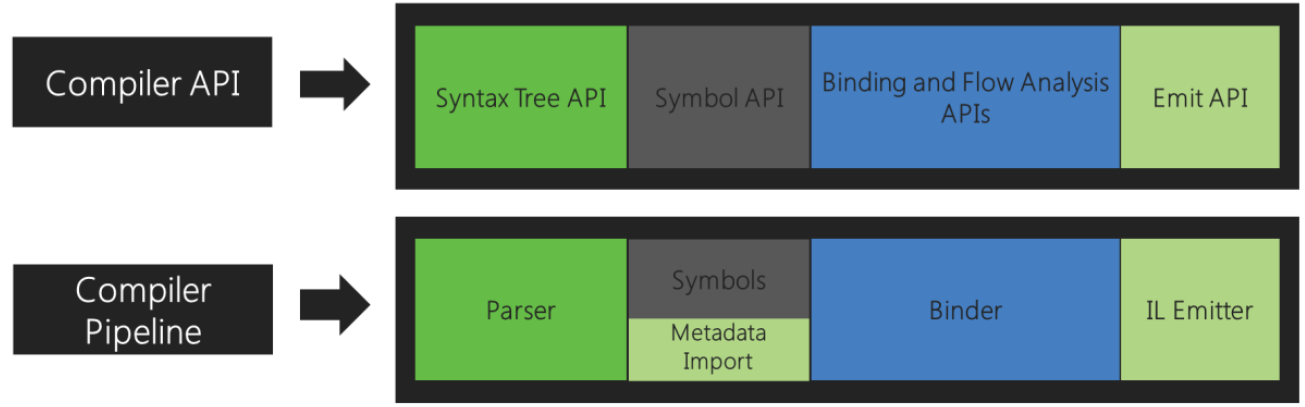
\includegraphics[width=1\textwidth]{\rootpath/worksheets/roslyn/figures/compiler_pipeline_vs_api} 
 \caption{Compiler pipeline in contrast to compiler \acp{API}\cite[p. 4]{ng2012roslyn}.}
\label{fig:api_vs_compiler_pipeline}
\end{figure}

Knowledge obtained through the \acp{API} is valuable in order to create tools that analyze and transform C\# or \ac{VB} code. Furthermore Roslyn allows interactive use of the languages using a \ac{REPL}\cite{cSharp2012interactive}, and embedding of  C\# and \ac{VB} in a \ac{DSL}\cite[p. 3]{ng2012roslyn}.

%\section{Roslyn Overview}\label{sec:inside_ros}\toby{Måske slet den her overskrift og ryk de indre sektioner en tak ud (fordi ellers skal syntax tree vel også ind under roslyn overview)}
%In this section we describe the architecture of Roslyn's source code and further elaborate on the compiler phases from \bsref{fig:api_vs_compiler_pipeline}. \toby{mere forklaring(indledning)}
%evt. skriv at den indre arktitektur skal give et overview, som gør det lettere at beskrive hvor de enkelte faser sker i koden i "compile phases"

\section{Roslyn Architecture}\label{sec:roslyn_archi}
\begin{figure}[htbp]
\centering
 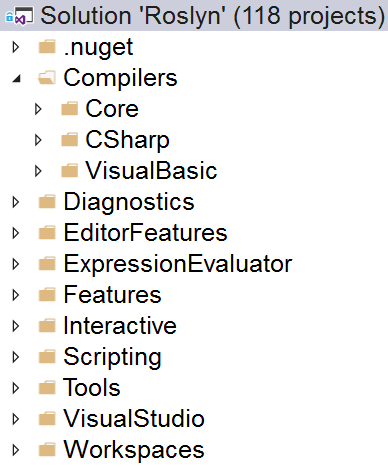
\includegraphics[width=0.4\textwidth]{\rootpath/worksheets/roslyn/figures/roslyn_solution_overview} 
 \caption{Overview of projects in Roslyn solution.}
\label{fig:roslyn_solution_overview}
\end{figure}

The Roslyn solution available on github\footnote{\url{https://github.com/dotnet/roslyn}}, forked\footnote{\url{https://github.com/Felorati/roslyn}} on the 9th February 2015, consists of 118 projects which include projects for Visual Studio development, interactive usage of the languages and more as illustrated on \bsref{fig:roslyn_solution_overview}. The focus in this report is on integrating \ac{STM} inside the Roslyn compiler as stated in \bsref{sec:problem_statement}\toby{skal det være en bsnameref?}, therefore we focus on the \bscode{Compilers} folder which contains the source code for the C\# and \ac{VB} compiler, each located in a separate folder. They share common code and functionality within the \bscode{Core} folder which includes code for controlling the overall compilation flow. As our scope is only on the C\# compiler, described in \bsref{sec:scope}\toby{skal det være en bsnameref?}, we describe only the C\# compiler and core code. However, the code for each compiler is very similar and use the same patterns for compilation\cite[09:36-10:36]{campbellDeeperRos}, so most of the following will apply for the \ac{VB} compiler also.

\begin{figure}[htbp]
\centering
 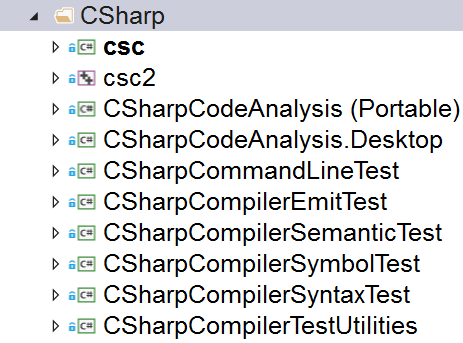
\includegraphics[width=0.4\textwidth]{\rootpath/worksheets/roslyn/figures/roslyn_csharp_overview} 
 \caption{Overview of CSharp folder.}
\label{fig:roslyn_csharp_overview}
\end{figure}

The projects contained in the \bscode{CSharp} folder are shown on \bsref{fig:roslyn_csharp_overview}. The \bscode{csc} project is the C\# command line compiler, which is the starting point of a C\# compilation. The \bscode{CSharpCodeAnalysis.Portable} and \bscode{CSharpCodeAnalysis.Desktop} projects contain the C\# code analysis, which is the actual code required for compilation. The rest of the projects in the \bscode{CSharp} folder mainly involve tests for the C\# compiler. The \bscode{Core} folder has similar to the \bscode{CSharp} folder, a  \bscode{CodeAnalysis.Portable} and \bscode{CodeAnalysis.Desktop} project which contain the common core analysis code.

\subsection{Overview of Compilation Call Chain}\label{ssec:overview_chain}
In \bsref{fig:roslyn_invoke_overview} an overview of the compilation call chain is shown. Compilation starts with \bscode{csc}'s main method being invoked, which calls the static \bscode{Run} method on the \bscode{Csc} class. This method creates a new \bscode{compiler} object of type \bscode{Csc}. \bscode{Csc} is a subtype of \bscode{CSharpCompiler}, located in the \bscode{CSharp.CSharpCodeAnalysis.Desktop} project, which again is a subtype of \bscode{CommonCompiler}, located in \bscode{Core.CodeAnalysis}. This means that the creation of the \bscode{compiler} object, calls the constructors of \bscode{Csc}, \bscode{CSharpCompiler} and \bscode{CommonCompiler}. Afterwards the \bscode{Run} method is invoked on the \bscode{compiler} object, which further invokes its parents \bscode{Run} method, which again invokes its parent \bscode{Run} method. Finally the \bscode{RunCore} method in \bscode{CommonCompiler} is invoked, which contains the general code that controls the overall flow of the compiler pipeline, illustrated in \bsref{fig:api_vs_compiler_pipeline}. The \bscode{RunCore} method will for the phases at run time call the specific compiler code for C\# in \bscode{CSharp.CSharpCodeAnalysis.Portable} or \ac{VB} in \bscode{VisualBasic.BasicCodeAnalysis.Portable} through dynamic dispatch.

\begin{sidewaysfigure}[htbp]
\centering
 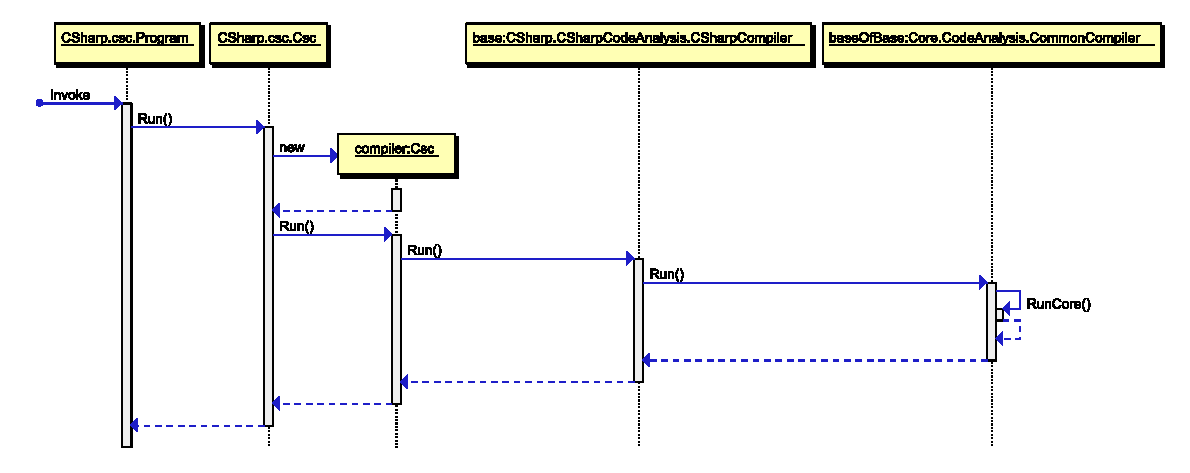
\includegraphics[width=\textwidth]{\rootpath/worksheets/roslyn/figures/seq_diagrams/roslyn_invoke_overview} 
 \caption{Sequence diagram showing an overview of the call chain of a C\# compilation.}
\label{fig:roslyn_invoke_overview}
\end{sidewaysfigure}

\section{Compile Phases}\label{sec:compile_phases}
The C\# compiler builds upon concepts from traditional compiler theory, such as lexing, parsing, declaration processing, semantic analysis and code generation\cite{sebestaProLang}\cite{fischer2009crafting}. Throughout the phases of compilation, traditional concepts such as a syntax tree, symbol table and visitor pattern\cite[p. 366]{gamma1994design} are also used. In this section we will elaborate on the compiler phases in the compiler pipeline shown in \bsref{fig:api_vs_compiler_pipeline}. In \bsref{fig:roslyn_csharpanalysis_overview} an overview of the folders inside the C\# code analysis is shown.

\begin{figure}[htbp]
\centering
 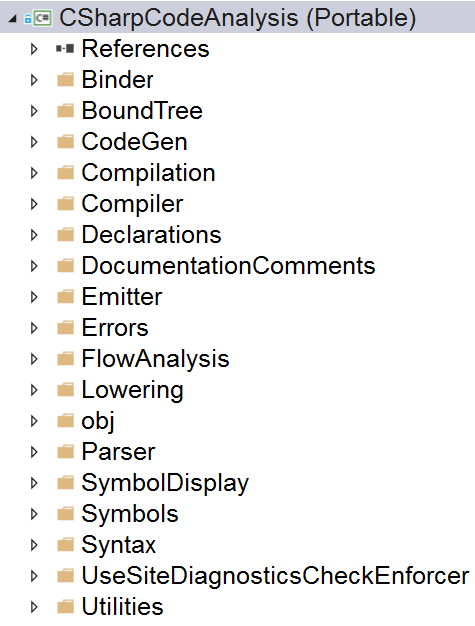
\includegraphics[width=0.4\textwidth]{\rootpath/worksheets/roslyn/figures/csharp_codeanalysis_overview} 
 \caption{Overview of the \bscode{CSharp.CSharpCodeAnalysis.Portable} project.}
\label{fig:roslyn_csharpanalysis_overview}
\end{figure}

\subsection{Initial Phase}
The initial phase of compilation entails initial work, such as parsing the command line with associated parameters and setting up for compilation, as described in \bsref{ssec:overview_chain}. This phase is executed sequentially\cite{sadovRoslynPerf}.

\subsection{First Phase}
\label{subsec:roslyn_first_phase}
The first phase involves parsing the source code, which is done in a traditional compiler fashion by lexing source code into tokens and parsing them into a syntax tree, which represents the syntactic structure of source code. The lexer is implemented using a \bscode{switch} used for identifying the type of token to lex given the first character of the token. The parser is implemented as a top-down parser using the common recursive descent approach. The parsing phase will check for syntax errors in source code, but does not have enough information to check for semantic errors, such as scope or type errors. The phase is concurrent, as several files may be parsed simultaneously\cite{sadovRoslynPerf}. The code for this phase is mainly located within the \bscode{Parser} and \bscode{Symbols} folder. We will describe the syntax tree and its contents in more detail in \bsref{sec:syntax_trees}.
\kasper[inline]{Måske lidt om at lexer og parser implementerings teknikker.}

\subsection{Second Phase}
\label{subsec:roslyn_second_phase}
The second phase involves creating a \bscode{Compilation} type object, specifically a \bscode{CSharpCompilation} type as we focus on the C\# compiler. A \bscode{Compilation} object contains information necessary for further compilation e.g. all assembly references, compiler options and source code. In the creation of a \bscode{CSharpCompilation} object, a declaration table is created which keeps track of type and namespace declarations in source code\cite{sadovRoslynPerf}. This is done sequentially\cite{sadovRoslynPerf}. Additionally the \bscode{Compilation} object contains a symbol table, which holds all symbols declared in source code or imported assemblies.\toby{Tror den er lazy, så først når den bruges laves den} Each namespace, type, method, property, field, event, parameter and local variable is represented as a symbol and stored in the symbol table\cite[p. 14]{ng2012roslyn}. Each type of symbol has its own symbol class, e.g. \bscode{MethodSymbol} derives from the base \bscode{Symbol} class. The symbol table can be accessed by the \bscode{GlobalNamespace} property, as a tree of symbols, rooted by the global namespace symbol. Furthermore there also exists a range of methods and properties to obtain symbols. The code for this phase is mainly located within the \bscode{Declarations} and \bscode{Symbols} folders.
%compilation is immutable, like syntax trees

\subsection{Third Phase}
In order to enable semantic analysis, the third phase entails fully binding all symbols, which is determining what each symbol actually refers to, e.g. what namespace and overloaded method, a particular method refers to. Any problems with symbol binding, like inheritance loops, will be reported. Binding is done concurrently, however binding members of a type will force base types to be bound also. For symbols not related, they can be bound in any order \cite{sadovRoslynPerf}.

Additionally, the binding phase also creates a bound tree, which is the Roslyn compilers internal tree used for flow analysis and emitting. In \cite{roslynBinder} Anthony D. Green states that they do not want to expose the bound tree through the \ac{API}: ``\textit{It has been a long standing design decision not to expose the bound tree. The shape of the bound nodes is actually pretty fragile compared to the shape of the syntax nodes and can be changed around a lot depending on what scenarios need to be addressed. We might store something somewhere one day for performance and remove it the next for compatibility or vice versa}''. Data flow and control flow analysis is employed, which uses the bound tree to e.g. check if statements are reachable, as the C\# specification states that an unreachable statement should produce a warning\cite{gafter2011}. The code for this phase is mainly located in the \bscode{Binder}, \bscode{BoundTree} and \bscode{FlowAnalysis} folders.

\subsection{Final Phase}
Finally, in the fourth and final phase all information built up so far is emitted as an assembly. Method bodies are compiled and emitted as IL concurrently, however methods within the same type are compiled sequentially in a fixed order, typically lexical ordering. The final emitting to the assembly is done sequentially.\cite{sadovRoslynPerf} The code for this phase is mainly located in the \bscode{CodeGen} and \bscode{Emitter} folders.

\section{Syntax Trees}\label{sec:syntax_trees}
Syntax trees are the primary structure used throughout compilation. Syntax trees of the Roslyn compiler have three key attributes\cite[p. 6]{ng2012roslyn}: 
\begin{enumerate}
	\item A syntax tree is a full fidelity representation of source code, which means that everything in the source code is represented as a node in the syntax tree. If programs are invalid, the syntax tree represents these errors in source code by tokens named \bscode{skipped} or \bscode{missing} in the tree.  This is referred to as being roundtripable.
	\item A syntax tree produced from parsing must be able to be translated back to the original source code.
	\item Syntax trees are immutable and thread-safe. This enables multiple users to use the same syntax tree at the same time in different threads without concurrency issues. As syntax trees are immutable, factory methods exist in order to help create and modify trees. Upon a modification, the factory methods does not copy the entire tree along with the modification, instead the underlying nodes are reused. This means that trees can be modified fast and with a low memory overhead. In fact a syntax tree in the Roslyn compiler consists of two trees, the red and green tree, which we will now describe.
\end{enumerate}

\subsection{Red And Green Trees}
\label{subsec:roslyn_red_green_trees}
The Roslyn team wanted a primary data structure for compilation with the following characteristics\cite{lippert2012redgreen}:
\begin{itemize}
	\item Immutable.
	\item Form of a tree.
	\item Cheap access to parent nodes from child nodes.
	\item Possible to map from a node in the tree to a character offset in the source code.
	\item Ability to reuse most nodes in the original tree when modifying trees.
\end{itemize}
However fitting all those characteristics into a single data structure is problematic\cite{lippert2012redgreen}:
\begin{itemize}
\item One problem is simply constructing a tree node, because both the child and parent are immutable and must have a reference to each other, so it is not possible to create one before the other.
\item Another problem is reusing nodes for other parents when modifying the tree, as nodes are immutable and it is therefore not allowed to change the parent of a node. 
\item A third problem is inserting a new character into the source code, as the position in source code of all nodes after that point changes. This is problematic in relation to adhering to the characteristic of reusing most nodes when modifying trees, because a modification to source code can change the character offset of many nodes.
%til den sidste, husk at de selv bruger roslyn til at udvikle interne værktøjer, derfor er det vigtigt at når man skrive et nyt tegn i starten af source koden, at de ikke skal bygge træet helt på nyt.
\end{itemize}

Instead the Roslyn compiler uses two types of trees, green trees and red trees, in order to fulfill all their requirements.

\paragraph{The green tree} is immutable, has the ability upon modification to reuse most unaffected nodes, has no parent references, is built bottom-up, and does not know the absolute positions of nodes in source code, only their widths\cite{lippert2012redgreen}.

For the expression ``5*5+5*5'', a typical parse tree is shown in \bsref{fig:normal_syntax_tree}, and a potential green tree is shown in \bsref{fig:green_syntax_deduplication}. As the green tree nodes do not have parent references and positions in source code, sub-trees and nodes can be reused, which results in a more compact tree. Factory methods are used to create new nodes in the tree in order to determine if existing nodes can be reused or new ones must be created. If nodes for a given expression already exist they are reused, otherwise new nodes are created. 

However reuse of existing nodes is not guaranteed, as that requires all nodes to be cached, which according to Vladimir Sadov in \bsref{sadovRoslynPerf} makes the reuse caches unnecessarily big. The caches are instead a fixed size, where new nodes will replace older ones when the max size is reached. Sadov states that it works pretty well because recently accessed nodes are likely to be accessed in the near future. Another trade-off is that they do not reuse non-terminals with more than 3 children, as it gets more expensive and less likely to match, the more children a non-terminal has\cite{sadovRoslynPerf}.

\begin{figure}[htbp]
\centering
 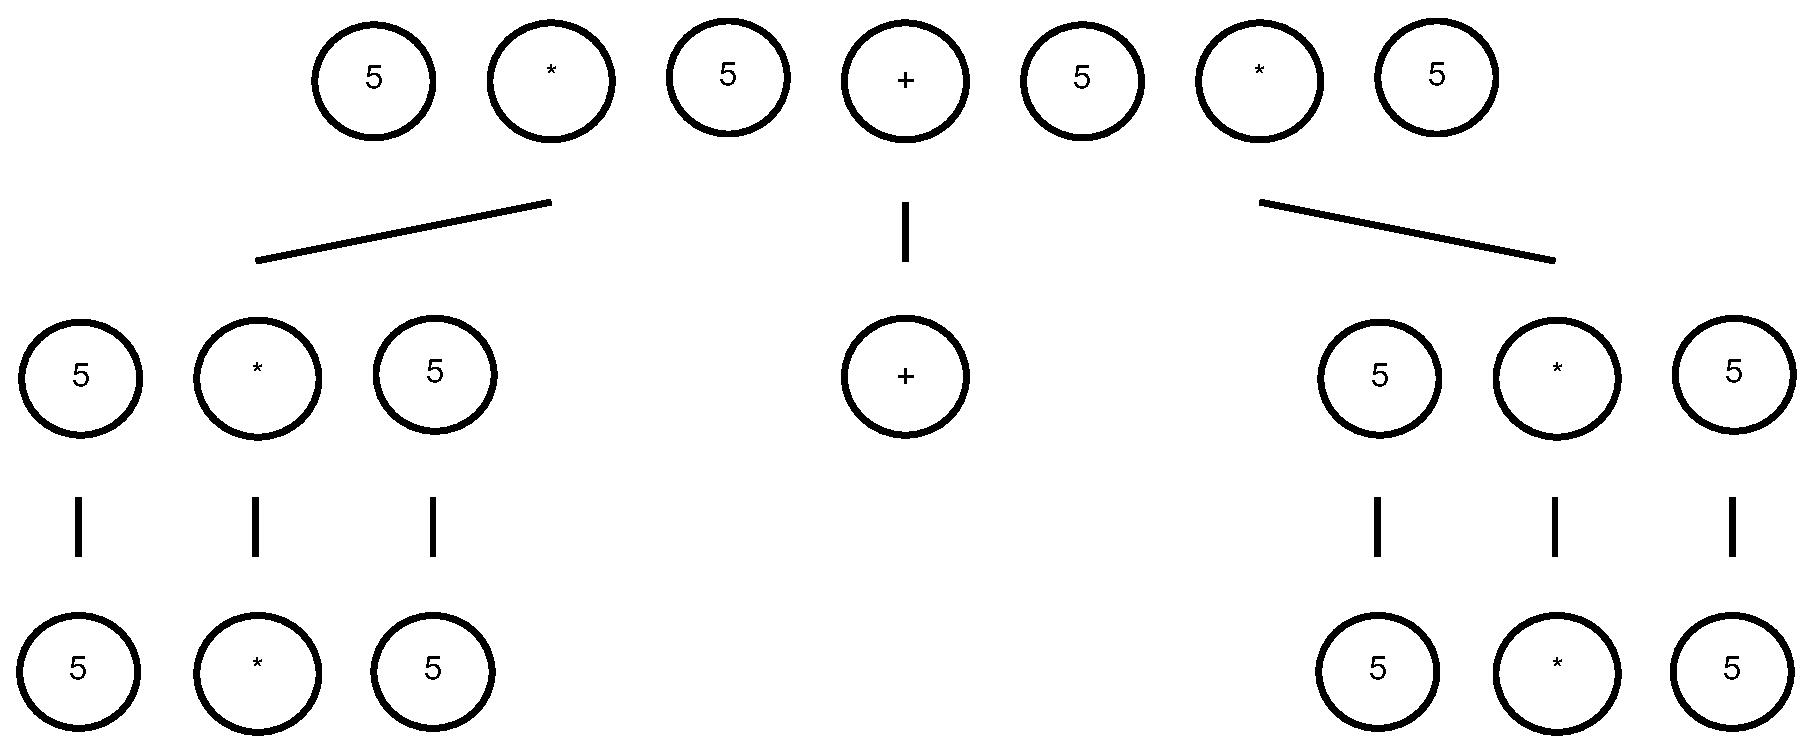
\includegraphics[width=\textwidth]{\rootpath/worksheets/roslyn/figures/normal_syntax_tree} 
 \caption{Typical parse tree of expression.}
\label{fig:normal_syntax_tree}
\end{figure}

\begin{figure}[htbp]
\centering
 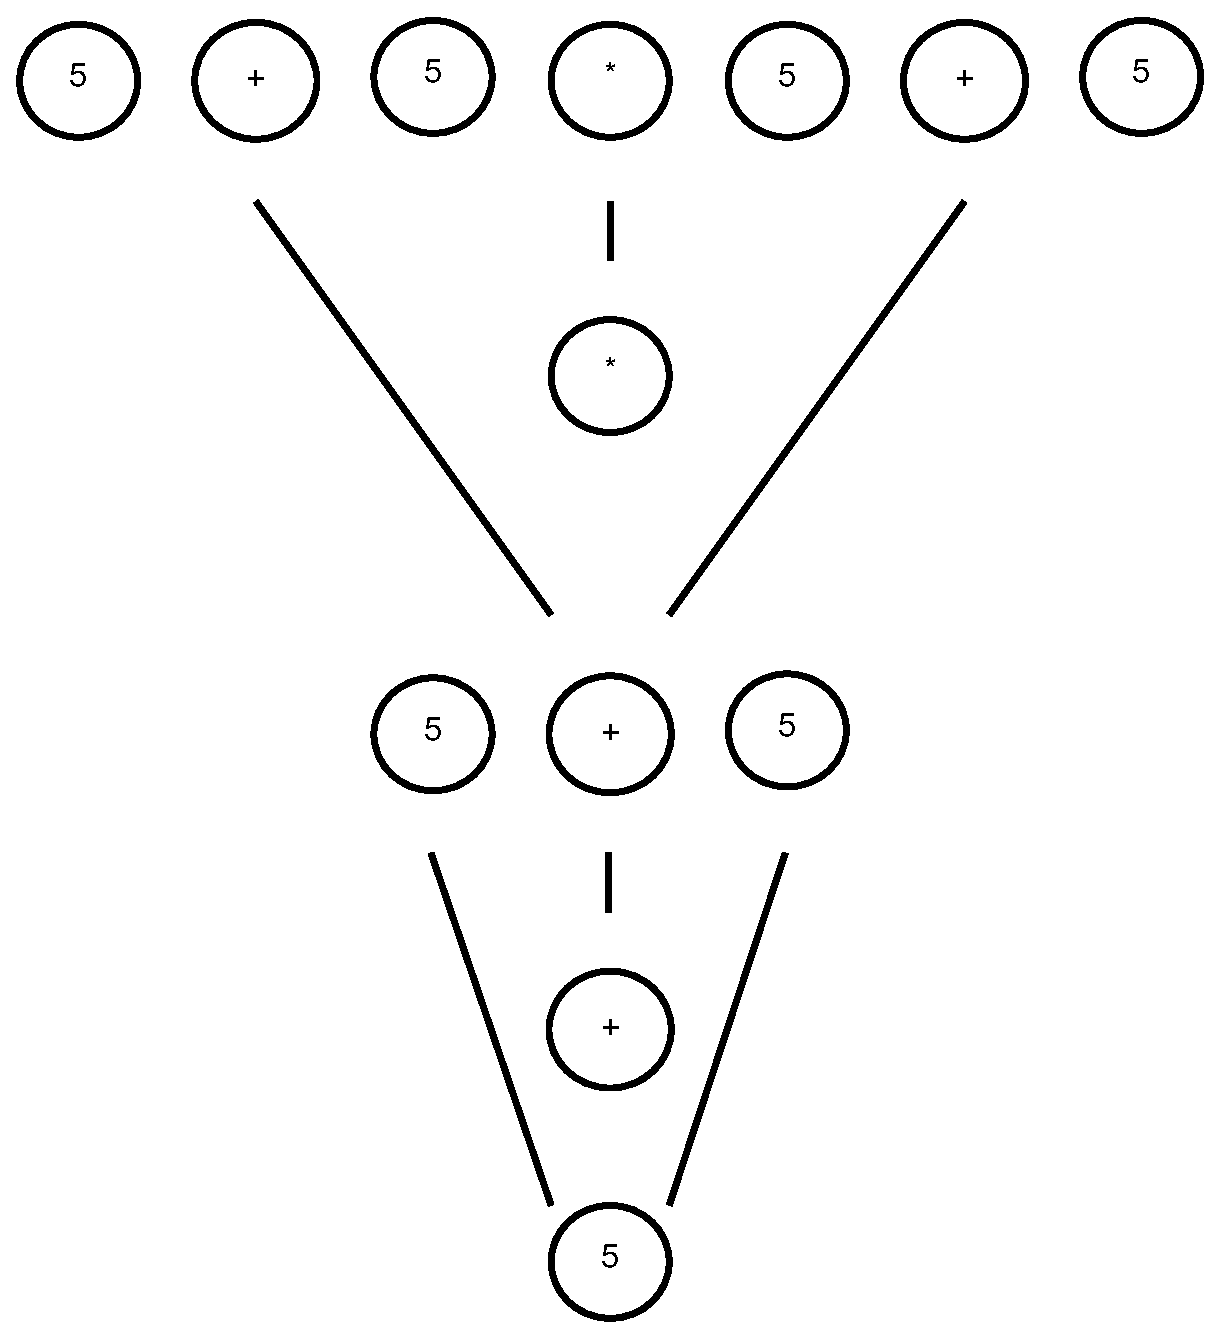
\includegraphics[width=0.6\textwidth]{\rootpath/worksheets/roslyn/figures/green_syntax_deduplication} 
 \caption{Green tree of expression, reusing identical sub-trees. Inspired by \cite{sadovRoslynPerf}.}
\label{fig:green_syntax_deduplication}
\end{figure}

\paragraph{The red tree} is an immutable facade built around the green tree. It has parent references and knows the absolute positions of nodes in source code. However these features prevent nodes from being reused, which means that making modifications to a red tree is expensive. Therefore they take another approach than building a new red tree upon every modification\cite{lippert2012redgreen}. 

The red tree is build lazily using a top-down approach, starting from the root of the tree and descending into children. To access a given node in the tree, the parent must first be available, otherwise the parents parent must be available, and so on. Once the parent of a node is available, all information required to construct a red node is available. The parent reference is known, as it is the current node. Additionally the internal data for the child can be obtained from the corresponding green node. Furthermore the absolute position of the node in source code can be computed, as the position of the parent is known, along with the source code width of all children that come before the given node\cite{sadovRoslynPerf}.

So when modifications are made to source code, an entire new red tree is not computed. Instead the green tree is modified, which is a relatively cheap operation, as most nodes can be reused. In terms of the red tree, a new root red node is created with 0 as position, null as parent and the root green node as the corresponding green node. The red tree will then only build itself if a user descends into its children, which may not happen and it might only descend into a small fraction of all the nodes in the tree\cite{sadovRoslynPerf}. % i forhold til hvad det er godt til? med ide typing tankegang

\subsection{Contents Of Syntax Trees}
The elements contained within syntax trees are syntax nodes, tokens and trivia. We will in this section describe these and some of their properties.

\subsubsection{Syntax Nodes}
Syntax nodes represent non-terminals of the language grammar, such as declarations, statements and expressions. It is one of the main elements of syntax trees and each syntax node type is represented as a separate class that derives from a base \bscode{SyntaxNode} class. As syntax nodes are non-terminals, they always have children, either in the form of other syntax nodes or syntax tokens. 

In relation to navigating syntax trees, all syntax nodes has\cite[p. 7]{ng2012roslyn}:
\begin{itemize}
\item A parent property to obtain the parent node
\item A child property for each child to obtain a given child
\item A \bscode{ChildNodes} method to return a list of all child nodes
\item Descendant methods i.e. \bscode{DescendantNodes}, \bscode{DescendantTokens} and \bscode{DescendantTrivia}, to obtain a list of all descendant nodes, tokens or trivia for a given node.
\end{itemize}

Additionally, optional children are allowed, which are represented as \bscode{null} if they are not present. For example an \bscode{IfStatementSyntax} syntax node has an optional \bscode{ElseClauseSyntax} syntax node\cite[p. 7]{ng2012roslyn}.

\subsubsection{Syntax Tokens}
Syntax tokens represent terminals of the language grammar, such as keywords, literals and identifiers. Opposed to syntax nodes, syntax tokens do not have any children. 

Each syntax token does not have a separate class, instead all syntax tokens are represented by a single \bscode{SyntaxToken} type. This means that there is a single structure for all tokens. To get the value of a token, there exist three properties: \bscode{Text}, \bscode{ValueText} and \bscode{Value}. The first returns the raw source text as a \bscode{String}, this includes extra characters such as escape characters. The second returns only the value of the token as a \bscode{String.} The last returns the value as the actual value type e.g. if the token is an integer literal then the property returns the actual integer. To allow different return types, the return type of the last property is \bscode{Object}\cite[p. 7-8]{ng2012roslyn}.

Additionally, for performance reasons the \bscode{SyntaxToken} type is defined as a struct, which is a value type\cite[p. 7]{ng2012roslyn}.

\subsubsection{Syntax Trivia}
Syntax trivia represent extra parts of source code that can appear between any two tokens, such as white space and comments. Syntax trivia is not included as a child node in the tree, but instead associated with a given token. In general, a token holds all trivia that follows it, on the same line, up to the next token. Syntax tokens hold trivia in two collections: \bscode{LeadingTrivia} and \bscode{TrailingTrivia}. The first token holds all leading initial trivia, and the end-of-file token holds the last trailing trivia in source code\cite[p. 8]{ng2012roslyn}.

As trivia are not nodes in the tree, they do not have a \bscode{Parent} property. Instead the associated token for some trivia, can be accessed with the \bscode{Token} property. Additionally, like syntax tokens, trivia's are also value types and have only a single \bscode{SyntaxTrivia} type to describe them all.

\subsubsection{Spans}
Every node, token and trivia knows its position in source code. This is accomplished by the use of a \bscode{TextSpan} struct type. A \bscode{TextSpan} object holds the start position of a node, token or trivia in source code and a count of how long it spans, both as 32-bit integers\cite[p. 8]{ng2012roslyn}.

Every node, token and trivia has two properties to obtain spans: \bscode{Span} and \bscode{FullSpan}. The \bscode{Span} property includes only the span of the node, token or trivia and not any trivia, where the \bscode{FullSpan} property includes the normal span and any leading or trailing trivia.  

\subsubsection{Kinds}
\label{subsubsec:roslyn_kinds}
Every node, token and trivia has an integer \bscode{RawKind} property, used to identify the syntax element type. Each language, C\# or \ac{VB}, then contains a \bscode{SyntaxKind} enumeration that contains all the nodes, tokens and trivia in the language, that the integer can be cast to. The \bscode{CSharpSyntaxKind} method does the casting automatically\cite{roslynwikiOverview}\cite[p. 9]{ng2012roslyn}.

Kinds are especially important for tokens and trivia, as they have only a single type, \bscode{SyntaxToken} and \bscode{SyntaxTrivia}, for all tokens and trivia. Thus, the only way to identify the particular token or trivia at hand, is by identifying its associated kind.

\subsubsection{Errors}
If programs are invalid as a result of errors in source code, a syntax tree is still produced. These errors are represented as special tokens in the syntax tree, which are added using one of the following techniques\cite[p. 9]{ng2012roslyn}.
\begin{enumerate}
\item Inserting a missing token in the syntax tree when the parser scans for a particular token but does not find it. The missing token represents the expected token, but it has an empty span and has a true \bscode{IsMissing} property.
\item Skipping tokens until the parser finds a token from where it can continue the parse. The skipped tokens are added as a trivia node with the \bscode{SkippedTokens} kind.
\end{enumerate}

\subsection{Syntax Tree Generation}
\label{subsec:roslyn_syntax_tree_generation}
The nodes, associated factory methods and visitor pattern implementation of the syntax tree is generated based on the contents of the \bscode{Syntax.xml} file located in the \bscode{CSharpCodeAnalysis (Portable)} project. The contents of the file describes information such as the fields and base class for each node in tree. Whenever the compiler is build, a tool, which source code resides in the \bscode{Tools\textbackslash CSharpSyntaxGenerator} project, generates the classes for each node defined in \bscode{Syntax.xml} along with relevant factory methods, properties for getting the value of each field associated with a node and pure methods for updating the fields of a node, that is generating a new node representing the change. The tool also generates the visitor pattern implementation along with the required \bscode{accept} methods on each node. Both the red and green tree, described in \bsref{subsec:roslyn_red_green_trees}, are generated during this process.




%EXTRA
%semantic model evt. (tror kun det er i forhold til api)
	%følgende sker direkte i runcore kald
%compilation = source files, assembly references and compiler options. Main: symbol table
	%består af symboler (Symbol klassen)
	
	%måske sker den semantiske analyse i analyzedriver kaldet, eller GetDeclarationDiagnostics()
%semantic model = semantisk analyse, så som type og scope checking, 
	%kan obtains udfra en compilation
	%MERE:
	%The symbols referenced at a specific location in source.
	%The resultant type of any expression.
	%All diagnostics, which are errors and warnings.
	%How variables flow in and out of regions of source.
	%The answers to more speculative questions.
	
%selve emitting sker også i runcore
	%data flow analyse, Control flow analysis også en del af emit (refer til deres paper det ligger på gitten omkring data flow)

%***EKSTRAAAA***
%dataflow og controlflow analyse sker også heri (nævn evt.)
%codegen, emitter og flowanalysis folders
%og i core: codegen og emitter (evt. skriv noget om corresponding i core, når jeg beskriver de to i csharp folderen. Eller deres corresponding base classes in core (hvilket ligger i de folere))

%***HUSK:
%også methodcompiler.cs i Compiler folder (sker faktisk inden endelig emitting)
	%bruger visitor pattern
%herefter controlflow pass (visistere bound tree)
%herefter dataflow pass

	
%CSharpCompilation GlobalNamespace

%Binder =  A Binder converts names in to symbols and syntax nodes into bound trees. It is context dependent, relative to a location in source code.

%second phase on fig 1.1 (tror jeg) - skal være sikker på hvad symbols er
%forklaret mere om den i CSharp > CSharpCodeAnalysis (Portable) > Declarations > Declaration.cs og DeclarationTable.cs (Table indeholder forskellige typer af Declaration, såsom SingleTypeDeclaration)

%second, declration phase: declarations from source and imported metadata are analyzed to form named symbols.
	%the declaration phase as a hierarchical symbol table
	%åbenbart både declaraiton og symbol table?

%***Mangler hvad fase 2 er i fig.1.1, eller hvor det sker præcist.

%*The fourth phase declaration diagnostics (fase 3 i fig 1.1)
%third phase of fig 1.1 (fully bind)
%resultatet er et bound træ, hvilket er en internal repræsentation for Roslyn (som ikke er tilgængelig igennemt API'et)
%symbol visitor sker heri (men den tager et symbol, så det må ske før)

%The fifth IL emitting
%the fourth

%The sixth serialization of portable executable file and pdb file (used for debugging).

%pdb info:
	%http://www.wintellect.com/devcenter/jrobbins/pdb-files-what-every-developer-must-know

%et sted skal scope og type tjek checkes

%secon phase on fig 1.1


%evt. lav en figur over disse faser

%sequential



%\toby[i]{Skal have det et sted, hvor jeg fortæller mere præcist en compiler line billedet om faserne der sker, ligesom beskrevet i blogpostet. Evt. også i forhold til om de køres med en eller flere tråde}
%Earlier in intro we looked at the phases of the compiler in contrast to the compiler API, howerver This does not include all phases. In this section we will explain in more detail what phases the compiler consits of and how it is build on in the code
	%Omformuler så det lyder bedere (men noget i den stil)

%Forklar de forskellige kompilerigns faser

%overordnet beskrivelse af faserne og evt. hvis api i forhold til også
	%ved ikke om jeg skal bruges deres tegning eller lave en ny selv (eller begge dele)

%snak ikke om det under white paper underskriften: API Layers

%MORE:

%Known Limitations and Unimplemented Language Features
	%https://social.msdn.microsoft.com/Forums/vstudio/en-US/f5adeaf0-49d0-42dc-861b-0f6ffd731825/known-limitations-and-unimplemented-language-features?forum=roslyn

%Liste over mulige emner:
	% Beskrivelse af kompileren, og hvad de muliggøre med deres API.
	% De enkelte faser i kompileren og generelt om dens opbygning
	% Hvilke ting de har gjort i forhold til at forbedre performance
	% Fortælle om deres røde og grønne syntaks træ
	% De anvender traditionel compiler teori, med lexer og parser + syntaxtræ og visitor til at traverserer træet. og emit fase.
	%Evt. fortæl om faserne i forhold til mapperne i projektet. Med Core, VB og C# projekternere og til sidst fortæl udfra C#'s mapper (og de forskellige faser).
	%Evt. også nævn syntax visualizer (nok ikke så vigtig, men er et værdifuldt værktøj)
	%Immutable data struktuerer!
	%Hvilke muligheder man har for at implementere STM direkte i Roslyn
		%Ved hjælp af API, hvor vi gør det først og derefter fodrer output til csc.exe
		%Direkte i compileren.


%Den primære brug der er tiltænkt at programmøren skal få adgang er gennem API laget, hvor en del kompleksitet stadig er gemt væk.
	%Vi vil gå direkte ind og ændre i selve compileren, hvilket ikke er tiltænk som hovedtanken fra Microsoft's side.
	
%Evt. skriv at vi vil have fokus på syntax træet og går mest i detalje med det, fordi vores implementering har valgt at ændre i syntax træet.
	%men alligevel kort om de andre faser.
\worksheetend